\documentclass[12pt, openright, twoside]{book}
% Some nonsense add
% <<<<<PACKAGES>>>>>
\usepackage[table]{xcolor}		% to shade cells in a table http://ctan.org/pkg/xcolor
\usepackage[utf8]{inputenc}
\usepackage{calc} % to perform arithmetic on the arguments of the LATEX commands \setcounter, \addtocounter, \setlength, and \addtolength

								% BIBLIOGRAPHY PACKAGES
\usepackage[backend=biber, style=numeric]{biblatex}
\addbibresource{doe.bib}

\usepackage{amsmath}			% MATHEMATICS PACKAGES
\usepackage{amsfonts}			%	V
\usepackage{amssymb}			%	V

\usepackage{chemfig}			% CHEMISTRY PACKAGES
\usepackage[version=4]{mhchem} 	%	V
\usepackage{chemformula}		%	V
\usepackage{chemmacros}			%	V
\usepackage{endiagram}			%	V
%\usepackage{mol2chemfig}		%	V


\usepackage[T1]{fontenc}		% FONTS
\usepackage{tgtermes} 			% body font
\usepackage{tgheros} 			% sans-serif font
\usepackage{inconsolata} 		% fixed width font
\usepackage{upgreek}			% to provide the upright Greek letters from the Euler or Adobe Symbol fonts as additional\\
								%	math symbols (\textbackslash\{\}upalpha, \textbackslash\{\}upbeta, etc.)

\usepackage{graphicx}			% for proper handling of graphicss included in the document
\usepackage{tabularx}			% for word-wrapping text in table columns
\usepackage{url}				% provides hyperliked urls throughout the document, useful for electronic copies
\usepackage{float}				% Improves the interface for defining floating objects such as 		figures and tables. 
\usepackage{booktabs}			% enhances the quality of tables in LATEX
\usepackage{makeidx}			% index sorting engine

\usepackage{dtk-logos}			% package for latex logos
\usepackage{rotating}			% package for rotating tables and figures
\usepackage{listings}			% package for allowing wrapping lines of verbatim text
\lstset{language=R,
	literate={<-}{{$\gets$}}1,
	breaklines=true,
	linewidth=\linewidth,
	basicstyle=\footnotesize,
	showspaces=false,
	showstringspaces=false}


%define page size and margins etc. 
\usepackage[paperwidth=6in, paperheight=9in]{geometry} 


\usepackage{fancyhdr} 			%to format headers and footers
\setlength{\headheight}{15.2pt}

\usepackage[hang,flushmargin]{footmisc}  % to not indent footnotes
\usepackage[small]{caption}  	% Captions and other tweaks - make caption text size smaller
\usepackage{tocloft}  			% to typeset table of contents
\usepackage[titletoc, header]{appendix}	% to properly display the Appendix in the TOC

%\usepackage[backref, colorlinks, bookmarks=true]{hyperref}
%\usepackage[cross, letter,center]{crop} %%Crop marks

\usepackage{verbatimbox}		% Control font size of verbatim text
\usepackage{pdfpages}			% Include pdf pages in a document
\usepackage{balance}			% to balance placement of floats for optimum output
\usepackage{booktabs}			% to enhance the quality of tables
\usepackage[all]{nowidow}		% to minimize orphans/widows on page breaks



\floatstyle{ruled} 
\restylefloat{figure}

% Invoke all modules of chemmacros
%\usechemmodule{all}

% preamble:
% uses siunits (loaded by endiagram)
\DeclareSIUnit{\calory}{cal}
\sisetup{per-mode = fraction}

\renewcommand*\oldstylenums[1]{{\fontfamily{Montserrat-TOsF}\selectfont #1}}


\setlength{\abovecaptionskip}{1.2ex}  %% Make space above and below captions smaller too
\setlength{\belowcaptionskip}{-1.5ex}


\newcommand{\allsectionsfont}{\normalfont\sffamily} % make section headers sans-serif to stand out
\newfloat{Structure}{tbp}{lop}	% define new float type for structures
\newfloat{Reaction}{tbp}{lop}	% define new float type for reactions


\let\oldverbatim\verbatim 		% make all verbatim (code blocks) text smaller, just for stylistic reasons
\renewcommand\verbatim{\small\oldverbatim}
\renewcommand{\cftchapfont}{\sffamily}
\renewcommand{\cftchappagefont}{\sffamily}
\renewcommand{\cfttoctitlefont}{\hfill\Huge\sffamily}  %format title of TOC to match chapter head format as set below:

%\includeonly{frontmatter, intro}

\setcounter{tocdepth}{2}		%% set level of header and subsection numbering is shown in TOC
\setcounter{secnumdepth}{2}
\author{Robert D. Solimeno}
\makeindex
\listfiles
\usepackage{hyperref}			% make pdf bookmarks with hyperlinks (problem child package list last)

% Image location
\graphicspath{{images/}}

%\overfullrule=2cm

\begin{document}
\frontmatter
% frontmatter.tex

% half-title page
\pagestyle{empty}
\vspace*{2in}
\begin{center}
{\Huge Statistics and Design Of Experiments for Chemists }
\end{center}

\newpage

% blank page
\
\pagestyle{empty}
 
\newpage
% title page
\vfill
\begin{flushleft}
	{\LARGE Robert D. Solimeno}
\end{flushleft}
\vfill
\begin{flushleft}
	\fontsize{50}{24.88}\textbf{Statistics and Design Of Experiments for Chemists}
\end{flushleft}
\vfill

\begin{flushleft}
	\includegraphics[scale=.35]{LogoBlackAndWhiteTextRight}
\end{flushleft}
\newpage

% copyright page
\noindent
Robert D. Solimeno\\
Immersitech LLC\\
Cincinnati, Ohio\\
USA\\
\textsf{rds@immersitech.com}\\

\vfill


Typeset by the author in \LaTeX{.} \\

ISBN -- XXX\\

\copyright 2018 Immersitech LLC
All rights reserved. This work may not be translated or copied in whole or in part without the written permission of the author, except for brief excerpts in connection with reviews or scholarly analysis. Any other use in any form of information, stored, retrieved, adapted electronically, computer software, by similar or dissimilar means known or unknown at the time of this writing is expressly forbidden.  The use in this publication of trade names, trademarks, service marks or other similar terms even if not identified as such, is not to be taken as the opinion whether or not they are subject to proprietary rights.
\pagestyle{empty}
\newpage
% dedication page
\begin{center}
\textsc{Dedication}
\end{center}
\vfill
\begin{center}
\textit{For my family far and near \dots}
\end{center}
\pagestyle{empty}
\vfill
\endinput
\tableofcontents \cleardoublepage
\listoffigures \cleardoublepage
\listoftables \cleardoublepage
% Introduction
\chapter{Introduction}

\section*{A toolbox for chemists}


\section*{How the book is organized}


\cleardoublepage

\mainmatter
% Setup Header and Foot styles for main document
\pagestyle{fancy} 				%use fancyheader

%% fiddle with chaptermark so we can make it not all caps
\renewcommand{\chaptermark}[1]{\markboth{#1}{}}
\renewcommand{\sectionmark}[1]{\markright{#1}{}}

%% get rid of any existing header and footer and header rule
\fancyhead{}
\fancyfoot{}
\renewcommand{\headrulewidth}{0pt}

% now make the footer the way we want it:
% page number on right side of footer for  odd pages
\rfoot[]{\small{\textsf{\hspace{0.25cm} \thepage}}}
\fancyhfoffset[EL]{0cm} %this looks like it doesn't do anything, but
%it seems to remind it to line up headers with
%the rest of the text

%page number and chapter name on left side of footer for even pages
\lfoot[\small{\textsf{\thepage \hspace{0.25cm} \leftmark}}]{}

\part{Introductory Statistics}
\chapter{Introduction}
\section{Population Statistics}

\textbf{Population statistics} \index{statistics!population} involve data from the entire universe of a subject under study.  For example, the population might consist of all the widgets ever produced and sold to customers. For  chemical producer it may comprise all of the historical physical property data for each product made.  In another circumstance one might deal with smaller, physical populations such as a specific lot of material produced at Factory ``A.''

All of the data elements are part of this universe and any calculated statistic is based on the entire population data set. Population statistics are denoted by Greek letters, e.g. $ \mu \ and \ \sigma $
\index{population}

\begin{center}
\begin{equation}
\mu  = average
\end{equation}
\end{center}

\begin{center}
\begin{equation}
\sigma  = standard \ deviation
\end{equation}
\end{center}

\index{average}\index{standard deviation}
\section{Sample Statistics}
In contrast, \textbf{Sample statistics} \index{statistics!sample} involve a relatively small sample of data taken from the population (universe) of data elements that belong to the entire population under study.  The sample data set is best selected in random fashion so that it adequately represents the characteristics of the whole population.

Sample statistics are denoted by English letters, and these statistics \textit{infer} what we can learn about the population.

\begin{center}
\begin{equation}
 \bar{x} = average \
\end{equation}

\begin{equation}
s = standard \ deviation
\end{equation}

\end{center}

Sample statistics are also known as \textsl{Inferential Statistics} \index{statistics!inferential}since they \textsl{infer} information about the population as a whole, based on the characteristics of a sample.  In this book we will deal exclusively with sample statistics, as this directly applies to the subject matter for the majority of chemical technologists.  In certain disciplines, genetics for example, population statistics are appropriately applied.  When in doubt, the use of sample statistics will be correct most of the time.

\section{Location versus Variation statistics}\index{location}

When one measures some \textsl{samples} from a \textsl{population}, then one may evaluate two types of statistics:

\begin{enumerate}
\item Location statistics, e.g. $ \bar{x} $ (average) and \index{statistics!location}
\item Variation statistics, e.g. $ s $ (standard deviation) \index{statistics!variation}
\end{enumerate}
\index{average}\index{standard deviation}
\subsection{Location Statistics}

Location statistics describe where the data are located, for example, on a number line.  Let's use an analogy that many people may relate to: pulling a car into a parking space or into a garage.  Ideally the driver wants to ``locate'' the vehicle in the center of the parking lane or the parking spot in the garage.  Each time a driver pulls into a parking spot though, the location is not always \textit{exactly} the same. There are several location statistics that can describe where the driver parks the vehicle \textit{most often}.

\subsubsection{Location statistics: Average}\index{average}
\index{statistics!location}
 
 There are at least three ways to express average:\index{average!mean}\index{average!median}\index{average!mode}
\begin{itemize}
  \item \textbf{Mean}:	sum $ n $ observations and divide by $ n $
  \item \textbf{Median}:	of $ n $ sorted observations, the $ n/2 $nd observation
  \item \textbf{Mode}:	the highest frequency observation of $ n $ observations
\end{itemize}

Location statistics \index{statistics!location} describe the tendency of a set of data to be located in a place of interest.  These can be described (as shown in the list above) by a most common location, most frequent, or at the mid-point of a range.

\index{location}

\begin{equation} \mu \index{mean} = Population \  mean\end{equation}

\begin{equation} \bar{x} =  Sample \  mean\end{equation}


\subsection{Variation Statistics} \index{statistics!variation}

Variation statistics describe how consistent (or not) a set of data may be around a location.  Once again using the parking space analogy from an earlier section, the variation statistic is like the maximum width of all of the attempts at pulling into the parking space.  How wide does a parking space need to be to accommodate the \textsl{average} driver?  This analogy is not precise, but it is convenient for a later topic about specification limits.  Nevertheless, it is assumed that the reader grasps the notion of variation here: how widely something varies about a given location.\index{location}

\subsubsection{Variation statistics: std dev \& range}
\index{standard deviation}\index{variance}  \index{statistics!variation} \index{standard deviation}
  \begin{itemize}
  \item Standard deviation, \textbf{s}   is a measure of how much a set of observations \textsl{vary}
  \item Variance is the square of standard deviation
  \item For a few observations, the range is easier to calculate and can be just as useful
  \end{itemize}
  
  
Formulas for population statistics:

\begin{center}
\begin{equation}
\sigma = \sqrt{\frac{1}{N}\displaystyle\sum_{i=1}^{N}{\left( x_{i}-\mu\right)}^2 }
\end{equation}

\begin{equation}
\sigma^{2} = {\frac{1}{N}\displaystyle\sum_{i=1}^{N}{\left( x_{i}-\mu\right)}^2 }
\end{equation}
\end{center}

Formulas for sample statistics:

\begin{center}
\begin{equation}
s = \sqrt{\frac{1}{n-1}\displaystyle\sum_{i=1}^{n}{\left( x_{i}-\mu\right)}^2 }
\end{equation}

\begin{equation}
s^{2} = {\frac{1}{n-1}\displaystyle\sum_{i=1}^{n}{\left( x_{i}-\mu\right)}^2 }
\end{equation}
\end{center}

where $ n $ corresponds to the sample size, e.g.  $ n = 5$.

\begin{center}
\begin{equation}
Range = max - min
\end{equation}

\end{center}
\index{range}
Remember this ... the example will help you remember what we are talking about:

 \begin{center}\textsl{\begin{Large}Pulling cars into a garage\end{Large}}\end{center}

\index{variation}
  \begin{itemize}
  \item How well the car is centered in the garage corresponds to its location, $ \bar{x} $
  \item How broadly the tire tracks appear on the floor corresponds to the variation, \textbf{\textit{s}}
  \item And the width of the garage itself corresponds to  \textit{specification limits} (more on this later)
  \end{itemize}
\index{location}
Hopefully this process is never out of specification!

\section{Accuracy \& Precision}
\subsection{Accuracy}
\index{accuracy}\index{precision}\index{average}
Accuracy is a measure of how close a measurement is to the true value of the property being measured.  The closer the (average) measured value is to the ''true value'' (usually unknown) reflects a higher degree of accuracy in the measurement.  One cannot rely on a single measurement so normal practice is to repeat measurements on a single sample or multiple samples (if the test is destructive) and to report the average value. Figure \ref{fig1} depicts accuracy versus precision graphically. The Central Limit Theorem states that:
\begin{quote}
conditions under which the sum of a sufficiently large number of independent random variables, each with finite mean and variance, will be approximately normally distributed.\cite{rice1995mathematical} \index{mean}
\end{quote}
\index{average}\index{variance}\index{variation}
Thus the average value of a ''sufficiently large number of independent random variables'' will tend to be closer to the true value than will any single observation.  This however, does not necessarily infer that the variation is small!

\begin{figure}[h]\caption{Accuracy versus Precision}\label{fig1}
\begin{center}
\includegraphics[scale=0.5]{accuracy-vs-precision}
\end{center}
\end{figure}

\subsection{Precision}
Precision is comprised of both \textit{repeatability} (same observer doing repeated measurements on the same or similar sample) and \textit{reproducibility} (different observers, sometimes on different equipment in different locations, doing repeated measurements on the same or similar samples).  It is a measure of the similarity in additional testing to assess both random and non-random sources of variation.  Random variation is something we all must live with ... but non-random variation has a root cause.  Once identified and quantified, the non-random variation can be reduced or eliminated.\index{variation}

\newpage
\section{Exercises}

\begin{enumerate}
\item Compare and contrast population statistics versus sample statistics.

\item What does the term \textit{inferential statistics} mean?

\item What is the difference between location statistics and variation statistics?

\item How are location statistics and variation statistics related to accuracy and precision?
\end{enumerate}



 
\chapter{Putting the basics to work}

\section{A typical work environment}
In a normal work environment, such as a biology, chemistry, or quality assurance lab most technicians already use some of the statistics covered in this text.  Taking a number of measurements, conveniently set to 3 or maybe 5 samples is the standard practice.  Reporting the mean value of a test result is already the norm.  Engineers also often collect data in the form of an observational study, or observed data are obtained through the analysis of historical observations.
\index{mean}\index{average}
Here's a synopsis of the typical situation:
\begin{center}
  \begin{itemize}
  \item Take a number of samples (depending on convenience of collection or available historical data)
  \item Do the measurement(s) and/or calculate average values
  \item Fill out a form (on paper or on the computer)
  \item Compare to the product specification(s)
  \item Decide whether the samples ''pass'' or ''fail'' the specification
  \end{itemize}
\end{center}  
  
Are both location and variation statistics considered here?  How does one actually decide whether the sample will ``pass'' or ``fail?''  If the (average) result just barely traverses a specification limit, does the production manager look at the raw data and seek one or more ``outliers?''  If the result is undesirable, does the analyst run the test again?\index{variation}\index{location}\index{average}
  
\section{Evaluating the quality of a process}
\index{variation}\index{location}\index{confidence}\index{t Distribution}
Fortunately, there is an unequivocal way to describe a result that cannot be refuted.  This method requires the use of both location and variation statistics and uses the \textit{Student's t Distribution} to calculate a \textit{confidence interval} as the criterion to establish if the result is significantly different -- \textit{statistically significant} -- at the desired level of confidence.

\subsection{Calculating the confidence interval}
\index{confidence}
\begin{center}
\begin{equation}
\bar{x} \pm t \cdot \frac{s}{\sqrt{N}}
\end{equation}
\end{center}

\textbf{Example: calculating the 95\% confidence interval}\\

Data: 7.5, 7.9, 8.3\\

$ \bar{x} $ = 7.9  s = 0.40\\

$ N = 3$, thus $(N-1)$ degrees of freedom = 2 \\

The value for $ t $ comes from a table of the Student’s $ t $ distribution by selecting the column of the table that corresponds with $ \alpha $ for the desired level of confidence, or $1-\alpha$ (in this case, 95\% confidence corresponds with $ \alpha = 0.05 $ -- two tails).  The row of the table corresponds to the $(N-1)$ degrees of freedom (in this case, 2 degrees of freedom). Using these values to select the correct column and row leads us to arrive at a value of: 4.303\\  (see Appendix \ref{AppendixA}).

\begin{center}
\begin{equation}
\bar{x} \pm 4.303 \cdot \frac{0.40}{\sqrt{3}}  =0.99
\end{equation}

\end{center}
\index{confidence}
The 95\% confidence interval is: $ 7.9 \pm \ 0.99 $\\

The method for communicating these results unequivocally is to state them as such: \textit{This laboratory is 95\% confident that the true value is between 6.91 and 8.89.}

NOTE: When an interval is calculated as in the example above, it must be understood that the \textit{true value} (that is always elusive and unknown) \textit{can be anywhere within that interval}.

\subsection{Does the product meet specification?}

Now that measurements have been made, and basic statistics have been calculated, a decision must be made to determine if specification criteria have been met.  Continuing with the example from above, let's assume the lower and  upper specification limits are set at the following values:

\begin{center}
\begin{equation}
LSL = 6.9  \hspace{0.5in}  USL = 8.9 
\end{equation}

\end{center}

Then we can depict the relationship between the confidence interval and the specification limits graphically (see Figure \ref{ConfInt}).
\begin{figure}[h]\caption{Representation of a measurement and 95\% C.I. within specification limits}\label{ConfInt}
\begin{center}
\includegraphics[scale=0.5]{spec1}
\end{center}
\end{figure}

This makes it obvious that the results indicate the product tested meets the specification criteria --- barely.  The 95\% confidence interval shown above is within the specification limits, but there is still a 5\% chance that the true value lies somewhere \textit{beyond} those limits.  In most cases this is an acceptable risk. In other circumstances where a failure could mean catastrophe or even loss of life, a higher degree of confidence is needed that results in a much wider interval.\\


Calculating the 99\% confidence interval:\\


The new value for $ t $  from a table of the Student’s $ t $ distribution: 9.925\\

\begin{center}
\begin{equation}
\bar{x} \pm 9.925 \cdot \frac{0.40}{\sqrt{3}}  = 2.292 
\end{equation}
\end{center}

The 99\% confidence interval is: $ 7.9 \pm \ 2.292 $\\


\textit{This laboratory is 99\% confident that the true value is between 5.608 and 10.192.}\\

This new interval in relation to the specification limits looks like that shown in Figure \ref{SpecLim}:

\begin{figure}[h]\caption{Representation of a measurement and 99\% C.I. traversing specification limits}\label{SpecLim}
\begin{center}
\includegraphics[scale=0.5]{spec2}
\end{center}
\end{figure}

Just as obvious as in the previous case, if this were a mission critical specification the test result clearly shows that the product does not meet the performance criteria.  Whenever a confidence interval traverses a specification limit, even if it is only one-sided, then one must conclude that the specification is not met.  Proper selection of the confidence level will provide the tolerable risk of having an incorrect conclusion.  
\newpage
\section{Exercises}
\begin{enumerate}
\item Describe a work environment from your past experiences in which data were collected, some analysis done, and results reported.  Specify how the data were reported, number of samples evaluated, calculations performed, etc.

\item What is a \textit{confidence interval}?

\item How does one find the correct value for $ t $ in a table of the Student's t distribution (see Appendix \ref{AppendixA})?

\item When reporting a result with 95\% confidence, what is the chance that this statement is wrong?
\end{enumerate}

\chapter{Hypothesis Testing}
\section{Statistical Hypotheses}\index{mean}\index{standard deviation}\index{confidence}\index{hypothesis}
In the previous chapters we discussed how to calculate the mean and standard deviation and to unequivocally state the value of a measurement (or series of measurements) at a desired confidence level.  Many technical problems involve the determination of whether to accept or reject a statement about some measured parameter.  For example, does the result given in the previous chapter help the technologist decide if it meets a specification limit?  In these circumstances a hypothesis is stated, and the decision making process about the hypothesis is called hypothesis testing.

This is perhaps one of the most useful aspects of inferential statistics since many types of technical problems involving decision making can be formulated in terms of a hypothesis statement. The hypothesis can be tested at a desired level of confidence to either accept or reject it based on numerical results.

\section{Pass or Fail?}\index{variation}\index{location}\index{confidence}\index{hypothesis}
As the lab technologist you have run multiple measurements, calculated the location and variation statistics, and determined the desired confidence interval.  Does the sample pass or fail the manufacturing specification?  Hypothesis testing (sometimes also known as a significance test) is the tool of inferential statistics that will help you make an affirmative statement.

\section{Types of data}
In order to properly choose the proper ``tool'' we must first decide the kind of data that we have. There are two different types of data:
\begin{enumerate}
\item Attribute data: things that are \textit{counted} as discrete events (e.g. defects, number of copier jams or mis\-feeds, etc.)
\item Continuous data: things that are measured on a continuously variable scale (e.g. \% moisture, thickness, mass, length, etc.)
\end{enumerate}



\index{null hypothesis}
\begin{table}\caption{Null Hypotheses for Discrete Data}\label{NullHypDisc}
\begin{center}
	{\renewcommand{\arraystretch}{1.8} %<- modify value to suit your needs
\begin{tabular}{|c|c|}
\hline \textbf{Test} & \textbf{Null Hypothesis}, $H_{o}$  \\ 
\hline 1 proportion & $\%Population =  ''Value'' $\\ 
\hline 2 proportions & $\%Population_{1} = \%Population_{2}$ \\ 
\hline 
\end{tabular} }
\end{center}
\end{table}

\subsection{Attribute Data}
As noted earlier, attribute data is that which is \textit{counted}. It is simpler to gather since it can be binary (yes/no or pass/fail). Attribute data has less resolution, since we only count if something occurs, rather than taking a measurement to determine the value of a continuously variable parameter. For example, attribute data for a manufacturing process might include the number of product defects (such as dents, or perhaps paint blemishes), whereas variable data for the same process might be the measurement of a critical product dimension, such as width or diameter.

Thus, attributes generally provide less information than measurement (variable) data would for the same process. Thus for attributes data, it is not readily predictable if the process is trending towards an undesirable state, since it is already in a discrete (pass/fail) condition. For this type of data the tests and null hypotheses are given in Table \ref{NullHypDisc}.\\

\index{mean}\index{variance}\index{null hypothesis}
\begin{sidewaystable}\caption{Null Hypotheses for Continuous Data}\label{NullHypCont}
\begin{center}
	{\renewcommand{\arraystretch}{1.8} %<- modify value to suit your needs
\begin{tabular}{|l|l|}
\hline \textbf{Test} & \textbf{Null Hypothesis}, $H_{o}$ \\ 
\hline 1-sample t-test & $\mu_{1} = value$ \\ 
\hline 2-sample t-test (independent samples) & $\mu_{1} = \mu_{2}$ two population means are equal \\ 
\hline paired t-test (dependent samples) & $\mu_{1} = \mu_{2}$ \\ 
\hline 1 way ANOVA & $\mu_{1} = \mu_{2}$  \dots $= \mu_{k}$ \\ 
\hline 1 variance, $\sigma^{2}$ &  $ \sigma =  value$ \\ 
\hline 2 variance & $\sigma_{1} = \sigma_{2}$ \\ 
\hline equal variances & $\sigma_{1} = \sigma_{2}$ \dots $= \sigma_{k}$  \\ 
\hline normality & population \underline{is normal} \\ 
\hline correlation (linear relationship only) & populations \underline{are not} correlated  \\ 
\hline 
\end{tabular} }
\end{center}
\end{sidewaystable}

\subsection{Variable data}
Variables data is acquired through continuously ``variable'' measurements, such as length, width, height, time, diameter, strength, weight, density, thickness, pressure, and temperature. It is quantitative. The degree of accuracy can be controlled by the appropriate choice of measuring device. For example, dimensions of length or diameter can be measured to the nearest 1/8th inch, millimeter, or micron depending on the measuring tool chosen. Variable data, also known as continuous data, are evaluated using the tests and null hypotheses found in Table \ref{NullHypCont}.


\section{Six steps to hypothesis testing}\index{hypothesis}
There are six steps to take in order to make the appropriate test for any particular situation:
\index{null hypothesis}
\begin{enumerate}
\item Have an idea
\item Translate the idea into statistical terms
\item Choose the Test whose null hypothesis $ H_{o} $ either agrees with or contradicts the \textbf{idea}
\item Sampling Step -- Determine the sample size and gather data
\item Analyze: find the p-value 
\item Decision: if p is low, reject $ H_{o} $
\end{enumerate}

\subsection{Have an idea}

This is a basic first step to define what question you desire to answer.  The ``idea'' needs to be developed and stated such that a question can be appropriately answered.  For example, a cereal manufacturer wants to determine whether the box filling process is on target.  The target fill weight for (the population of) cereal boxes is 365 grams.

One can state the ``idea'' for this situation as such: ``The average (mean) fill weight for cereal boxes is 365 grams.''
\index{mean}\index{average}

\subsection{Translate the idea into statistical terms}

Now that the idea has been articulated, one can translate this into statistical terms. In this example we can state the situation as such:

\begin{center}
\begin{equation}
\mu = 365 g
\end{equation}
\end{center}


\subsection{Choose the Test}
\index{null hypothesis}\index{hypothesis}
The next step in hypothesis testing is to choose the appropriate test.  The way to do this is very straight-forward:  choose the test whose null hypothesis, $H_{o}$, either agrees with or contradicts the IDEA.  From the section above, we stated the IDEA to be $ \mu = 365 g $, and this form of a null hypothesis, e.g. $ \mu = $ \textit{value} (where \textit{value} is given by the study) equates to the 1-sample t-test.  

\subsection{Sampling Step}
At this step in the process it is time to decide how many samples are to be taken, how they will be taken (or document how they already have been taken), and what measurements will need to be taken.  It is good practice to standardize routine tasks by developing a data record form, either paper or electronic, to facilitate and error-proof as much as possible the data collection process.  In many cases there is abundant historical data to sift through.  In some circumstances though, fresh observations need to be collected and this step may be the most laborious step.  If this is the case, the standardization of data entry mentioned above will serve this situation well.

\subsection{Analyze}\index{mean}\index{standard deviation}
Calculation of means and standard deviations are carried out in this step.  The real analysis takes place by means of determining the $p-value$ which can often be done by referring to a t-table in the appendix of a textbook (see also Appendix \ref{AppendixA}). Finding the $p-value$ requires a ''backward'' use of the table -- finding the t-value in the table and then looking up the $p-value$ at the top of the appropriate column.  However, interpolation is most often required. Statistical software can be applied to give immediate and precise results at minimal effort.

\begin{table}
	\begin{center}
		{\scriptsize 
			\begin{tabular}{llllllll}
			\toprule
			\textbf{Variable} & \textbf{N} & \textbf{Mean} & \textbf{Std Dev} & \textbf{SE Mean} & \textbf{95\% CI} & \textbf{T} & \textbf{P} \\
			\midrule
			Box Weight & 6 & 366.705 & 2.403 & 0.981 & (364.183, 369.226) & 1.74 & 0.143 \\ 
%			\bottomrule
			\end{tabular} 
		}
\end{center}
	\caption{1-sample t-test result for an example, the test of $ \mu = 365 g $ }\label{1samplet} \index{mean}
\end{table}


\subsection{Decision}\index{null hypothesis}
Now it is time to interpret the results and render a decision.  To decide, one must choose the significance level, $\alpha$ (alpha) before doing the test.  In this case $\alpha = 0.05$ which is a common value used for many tests.  Different values can be chosen -- higher or lower -- depending on the sensitivity required for the test and the consequences of incorrectly rejecting the null hypothesis.  Yes, there is some risk here!  But the analyst can choose the level of risk that is reasonable and tolerable for the given situation.  In many cases, the $\alpha = 0.05$ significance level is quite appropriate.

Therefore, based on $\alpha = 0.05$ one compares the $p-value$ to $\alpha$ -- and the decision is made as such: \textit{if P is low (less than or equal to $\alpha$), reject $H_{o}$.}

\begin{center}
\LARGE If P is low, reject $H_{o}$.
\end{center}
\index{confidence}\index{null hypothesis}
So what if P is not low, as in the case above ($p = 0.143$)?  Then we ``fail to reject'' the null hypothesis - in other words ``we don't really know.''  Significance tests only provide evidence when refuting the null hypothesis.  In cases such as this when the null hypothesis cannot be rejected, ``we don't really know'' in the strictest statistical sense. So in this example, we cannot refute the hypothesis that  $ \mu = 365 g $ - however we can't go so far to affirm that indeed  $ \mu = 365 g $, we simply cannot reject this hypothesis at the 95\% level of confidence.\\

\subsection{Power}
There is a possibility that the result of a statistical test such as this will not reject the null hypothesis when a real difference truly exists.  This is called a ``Type II error'' -- or ''False Negative.''  This \textit{possibility}, or more precisely this \textbf{probability} is $ \beta $, and thus

\begin{center}
\begin{equation}
Power = 1 - \beta
\end{equation} 
\end{center}
 Therefore, \textbf{Power} is the probability of detecting a difference in between two populations \textit{when one truly exists}. Bigger effects are easier to detect, obviously. In the case postulated above in which a Type II error is suspect, it is possible that the Power was insufficient to discern a real, but perhaps smallish effect.  To decrease the chance of a Type II error one must increase the statistical Power of the test.  Usually this is achieved by increasing $N$ (i.e. taking more samples).
\index{confidence}
\begin{table}[h]\caption{Significance test result matrix}\label{SigTest}
\begin{center}
		{\renewcommand{\arraystretch}{1.8} %<- modify value to suit your needs
\begin{tabular}{|l|l|}
\hline   Do Not Reject $H_{o}$  &  Do Not Reject $H_{o}$   \\
 $p = 1-\alpha = $ Confidence & $p = \beta = 1-Power$ \\
  \textbf{GOOD} & \textbf{BAD} -- ''Type II error'' \\
  & ''False Negative'' \\
\hline Reject $H_{o}$ & Reject $H_{o}$ \\
 $ p = \alpha$ & $p= Power = f(\alpha, N, \sigma, d)$  \\
 \textbf{BAD} -- ''Type I error''    & \textbf{GOOD} \\
 ''False Positive''  &  \\
\hline 
\end{tabular} }
\end{center}
\end{table}

\section{Using R statistical software}
R is a free software environment for statistical computing and graphics.\cite{Venables2012}\cite{Mohr2018} R is available as Free Software under the terms of the Free Software Foundation’s GNU General Public License in source code form. It compiles and runs on a wide variety of UNIX platforms and similar systems (including FreeBSD and Linux), Windows and MacOS. The software provides a wide variety of statistical and graphical techniques. When paired with RStudio, an integrated development environment (IDE), development of code to analyze a wide variety of statistical analyses is made easy.

The RStudio IDE provides a command console to execute individual R commands, just like a native R session. In addition, the IDE provides an editor that offers syntax highlighting, code completion, and smart indentation. The R code entered into the editor can also be executed directly from the source editor. Interested readers can see more information about RStudio and download a free version at \url{https://www.rstudio.com/products/RStudio/}.

To demonstrate using R, let's compute statistical power -- discussed in the previous section.  Assuming we have a ``medium-sized'' effect where a 0.5 unit shift can be detected. We want our significance level to be $\alpha = 0.05$ and we have resources to test 50 samples of each population for comparison. Computing power in R would require the \emph{pwr} package which should already be loaded, and then the following code would produce:

\begin{lstlisting}
> #Example of an analysis to find the power to detect a medium sized effect give 50 samples per cell (100 samples total)
  
> pwr.t.test(n = 50, d = .5, sig.level = .05, power = NULL, alternative = "two.sided", type = "two.sample")
\end{lstlisting}

\noindent\textbf{Output:}\\
\texttt{Two-sample t test power calculation }

\noindent\texttt{n = 50
d = 0.5
sig.level = 0.05
power = 0.6968934
alternative = two.sided}

\noindent\texttt{NOTE: n is number in *each* group}\\


The ``NULL'' value assigned to power in the code example tells the software to compute that parameter. Any of the first four parameters (n, d, $\alpha$, power) can be computed by setting to NULL and providing the other three. The hypothesis test for the two samples of n=50 would give power of about 70\% at the 5\% significance level (i.e. 95\% confidence).

How many samples would be required to have 90\% power?

\begin{lstlisting}
> pwr.t.test(n = NULL, d = .5, sig.level = .05, power = .9, alternative = "two.sided", type = "two.sample")
\end{lstlisting}

\noindent\textbf{Output:}\\
\texttt{Two-sample t test power calculation} 

\noindent\texttt{n = 85.03128
d = 0.5
sig.level = 0.05
power = 0.9
alternative = two.sided}

\noindent\texttt{NOTE: n is number in *each* group}\\


The answer: 85 samples must be measured to achieve a power of 90\% - almost double the number of samples required at 70\% power.
\newpage
\section{Exercises}

\begin{enumerate}
\item Are these samples the same or are they different?

\begin{tabular}{|c|c|}
\hline \textbf{Sample 1} & \textbf{Sample 2} \\ 
\hline 14.59 & 14.62 \\ 
\hline 15.01 & 14.69 \\ 
\hline 15.47 & 14.95 \\ 
\hline 15.56 & 14.76 \\ 
\hline 15.05 & 14.87 \\ 
\hline 

\end{tabular}\\
\index{confidence}
\item Calculate $ \bar{x}, s, $ and 95\% confidence intervals for \textbf{Sample 1} and \textbf{Sample 2} from the table above.
\item Plot the mean values using a line chart (\textbf{Sample 1}, \textbf{Sample 2}, and \textbf{Sample 3} from the table below) with 95\% confidence intervals as error bars.\index{mean}

\begin{tabular}{|r|r|r|r|}
\hline Obs. & \textbf{Sample 1} & \textbf{Sample 2} & \textbf{Sample 3} \\ 
\hline 1 & 7.5 & 7.2 & 7.7 \\ 
\hline 2 & 7.9 & 7.4 & 7.9 \\ 
\hline 3 & 8.3 & 6.9 & 8.3 \\ 
\hline 
\end{tabular} 

\end{enumerate}

\part{Design of Experiments}
% Intro to DOE
\chapter{Introduction to DOE}
This short course is an introduction to experimental design, also known as ''design of experiments'' -- abbreviated \textit{DOE}. Students will learn the value of applying experimental design principles versus a one-factor-at-a-time approach. Full factorial and fractional factorial designs are covered with in-class experiments using this methodology.

Performing an experiment is basically a test to see how the process, instrument, or device \textit{responds} to deliberate changes in a number of settings, or \textit{factors}.  The investigator's interest is in observing how the deliberate changes of the input variables (factors) affect the output variables (responses).  In the analysis of the experimental data the investigator may identify reasons for changes in the responses such that a better understanding of the system under study is achieved.

Planning and conducting experiments in a structured way and analyzing the results of such a study provide for valid and objective conclusions to be made.  The strategies used in this type of experimentation reveal to what extent a variety of factors influence the responses of interest, and in addition also reveal if there are any \textit{interaction}  effects between the factors that are significant.

The alternative strategy of experimentation that is widely practiced is the one-factor-at-a-time approach. In this method a base set of levels for each factor is established, and then each factor is varied over its range while all other levels are held constant. Graphical analysis is typically used to compare the responses for each factor to each other when varied over the range of interest with all others being held constant. The major disadvantage of this approach is that it fails to consider any possible interaction between the factors.  Interactions between factors are very common!

The correct approach in dealing with multiple input settings is to conduct a \textbf{factorial experiment} in which \textit{the settings are varied together} instead of one at a time.  This experimental design concept is of crucial importance and the detailed examples and exercises that follow will serve to demonstrate how to carry out such a plan, how to analyze the data, and interpret the results.
% Full Factorial Designs
\chapter{Full Factorial Designs}

\section{Learning by experimentation}
We do experiments to test a hypothesis -- something we think might be true but have no evidence to demonstrate the idea.  The process of experimentation is a \textit{learning} process.  The experiments that this course offers for study are those that are intended to improve the quality of product designs and production (or measurement) processes.

To ''improve the quality'' means:

\begin{itemize}
\item Optimizing the mean value of response(s) -- a traditional focus of experimental designs.  For example, maximize yield of a chemical reaction, optimizing the opacity of printing paper, or maximizing the distance a catapult launches a projectile. In each of these examples there are various settings involved in making the process work that may be adjusted to different levels or settings.  Adjustment of these parameters in relation to each other can achieve the desired end result -- and is the object of the experiment.

\item Minimizing variation in a process or product -- variation and quality of performance are inversely related. There is always some variation present in any process, i.e. random variation that is uncontrollable, and the role of experimentation in reducing variation is to identify and reduce those sources of variation that are not random and are controllable.
\end{itemize}

The definition of an experiment used here is a series of trials or tests that produce quantifiable outcomes. While the criterion for quantifiable outcomes is established, the initial data need not be numerical results. Pass/fail results, or categorical results established with Excellent/Good/Fair/Poor judgements can be converted to numerical results by assigning values to each category.

\section{Traditional methods}
Some scientists or engineers with many years of experience might say, "I know how to test products - just vary one thing at a time and keep everything else constant so you can see the effect of what you are changing."  While one variable at a time experiments have an intuitive appeal and seem quite straight-forward to plan and do, they are not good experiment designs.  These types of experiments generally:

\begin{enumerate}
\item lead to misleading conclusions,
\item cannot reveal any possible interaction effects,
\item may not result in determining the true optimum conditions, and
\item are usually inefficient.
\end{enumerate}

There is a better way.  Factorial experiments are those in which every level of one factor is run in combination with all levels of the other factors.  Thus all possible combinations are run in a factorial design experiment. It should be understood that the factors being studied in these types of experiments are \textit{independent variables}.  These are usually process settings such as temperature, line speed, tool size, material substitution, etc.  

For experiments with many factors this can lead to a large number of runs, or tests.  There are several ways of dealing with these situations to reduce the number of runs in the factorial experiment while preserving all of the useful information. These methods are dealt with in the next chapter.

\section{Two-factor design}
\begin{table}[h] \caption{The $ 2^{2} $ factorial design }\label{tab1}
\begin{center}
\begin{tabular}{|l|c|c|}
\hline Run & A & B \\ 
\hline 1 & -- & -- \\ 
\hline 2 & -- & \cellcolor{black!25}+ \\ 
\hline 3 & \cellcolor{black!25}+ & -- \\ 
\hline 4 & \cellcolor{black!25}+ & \cellcolor{black!25}+ \\ 
\hline 
\end{tabular} 
\end{center}
\end{table}
The most common full factorial designs are two-level experiment designs denoted as $ 2^{n} $ designs, where $2$ denotes the number of levels for each factor to be evaluated and $n$ denotes the total number of factors under study.  The simplest of these is the 2-factor, 2-level design, or the $ 2^{2} $ design that involves 4 sets of conditions, or runs, to complete the experiment.  This number of experimental runs is determined by computing the exponential expression $ 2^{2} = 4 $.

In Table \ref{tab1}, the ''--'' denotes a low level of the corresponding factor (A or B) and the ''+'' denotes a high level of the factor.  Hence the name ''two-factor, two-level design'' where A and B are the two factors and ''--'' and ''+'' denote the two levels. In the example that follows we will run an experiment, collect individual observations of repeated runs, and analyze the data ``manually'' (and is easily done with spreadsheet software).

\subsection{EXAMPLE:The Pump Experiment} 
\label{router}
A diaphragm pump is one in which a diaphragm, made of or coated with a chemically resistant material (such as PTFE), is actuated in successive compression/decompression cycles to deliver liquid materials. The liquid does not penetrate through the diaphragm. The repeated compression/decompression changes the volume of a chamber in the pump head so that liquid enters through an inlet check valve during decompression and exits through an outlet check valve during compression, effectively pushing material through the chamber.   Two factors are presumed to have an influence on pump metering accuracy: the output check value spring size (Factor A), and  the pump speed (Factor B). These two factors are independent since each can be changed by a process operator without influencing the other factor, i.e. pump speed does not influence the check valve and vice-versa.

There are two pump speeds that can be used and two spring sizes that are reasonable.  Therefore there are four possible combinations as depicted in Table \ref{RoutDes}:

\begin{table}[]
	\begin{tabular}{rc|c|c|c|c|}
		\cline{3-6}
		\multicolumn{1}{c}{\textbf{}}                                                   & \multicolumn{1}{l|}{}                                        & \multicolumn{2}{c|}{\textbf{\begin{tabular}[c]{@{}c@{}}A\\ Pump  \\ Speed\end{tabular}}} & \multicolumn{2}{c|}{\textbf{\begin{tabular}[c]{@{}c@{}}B\\ Spring size\end{tabular}}} \\ \cline{3-6} 
		\multicolumn{1}{l}{}                                                            & \multicolumn{1}{l|}{}                                        & \textbf{-}                                      & \textbf{+}                                     & \textbf{-}                               & \textbf{+}                              \\ \hline
		\multicolumn{1}{|c|}{\begin{tabular}[c]{@{}c@{}}Std\\ Run\\ Order\end{tabular}} & \begin{tabular}[c]{@{}c@{}}Random\\ Run\\ Order\end{tabular} & 40 g/min                                          & 90 g/min                                         & 15 psi                                & 100 psi                                \\ \hline
		\multicolumn{1}{|r|}{\textbf{1}}                                                & \textbf{3}                                                   & \multicolumn{2}{c|}{40 g/min}                                                                      & \multicolumn{2}{c|}{15 psi}                                                     \\ \hline
		\multicolumn{1}{|r|}{\textbf{2}}                                                & \textbf{1}                                                   & \multicolumn{2}{c|}{40 g/min}                                                                      & \multicolumn{2}{c|}{100 psi}                                                      \\ \hline
		\multicolumn{1}{|r|}{\textbf{3}}                                                & \textbf{4}                                                   & \multicolumn{2}{c|}{90 g/min}                                                                      & \multicolumn{2}{c|}{15 psi}                                                     \\ \hline
		\multicolumn{1}{|r|}{\textbf{4}}                                                & \textbf{2}                                                   & \multicolumn{2}{c|}{90 g/min}                                                                      & \multicolumn{2}{c|}{100 psi}                                                      \\ \hline
	\end{tabular}\caption{Metering Pump Experiment Design}\label{RoutDes}
\end{table}








The experimenter has chosen to run four replicates of this experiment.  Four vessels are weighed at each run condition in the above table.  The data recorded is the mass of liquid delivered by the pump at the set speed and size of springs used. The goal of the experiment is to deliver a specific mass of material at the desired rate, and the response variable to be analyzed is the deviation in milligrams of the target mass delivered.. Table \ref{RouterData} summarizes the data collected.

\begin{table}[]
\begin{tabular}{lcc|r|r|r|r|r}
\cline{4-7}
                                                                                   & \multicolumn{1}{l}{}                                                                   & \multicolumn{1}{l|}{} & \multicolumn{4}{c|}{\textbf{Replicates}}                                                                                              & \multicolumn{1}{l}{}                                                                   \\ \hline
\multicolumn{1}{|c|}{\textbf{\begin{tabular}[c]{@{}c@{}}Run\\ Order\end{tabular}}} & \multicolumn{1}{c|}{\textbf{\begin{tabular}[c]{@{}c@{}}Cutting \\ Speed\end{tabular}}} & \textbf{Bit Size}     & \multicolumn{1}{c|}{\textbf{1}} & \multicolumn{1}{c|}{\textbf{2}} & \multicolumn{1}{c|}{\textbf{3}} & \multicolumn{1}{c|}{\textbf{4}} & \multicolumn{1}{c|}{\textbf{\begin{tabular}[c]{@{}c@{}}Mean \\ Response\end{tabular}}} \\ \hline
\multicolumn{1}{|l|}{1}                                                            & \multicolumn{1}{c|}{40 rpm}                                                            & 1/8th in              & 18.2                            & 18.9                            & 12.9                            & 14.4                            & \multicolumn{1}{r|}{16.1}                                                              \\ \hline
\multicolumn{1}{|l|}{2}                                                            & \multicolumn{1}{c|}{90 rpm}                                                            & 1/8th in              & 27.2                            & 24.0                            & 22.4                            & 22.5                            & \multicolumn{1}{r|}{24.0}                                                              \\ \hline
\multicolumn{1}{|l|}{3}                                                            & \multicolumn{1}{c|}{40 rpm}                                                            & 1/16th in             & 15.9                            & 14.5                            & 15.1                            & 14.2                            & \multicolumn{1}{r|}{14.9}                                                              \\ \hline
\multicolumn{1}{|l|}{4}                                                            & \multicolumn{1}{c|}{90 rpm}                                                            & 1/16th in             & 41.0                            & 43.9                            & 36.3                            & 39.9                            & \multicolumn{1}{r|}{40.3}                                                              \\ \hline
\end{tabular}\caption{Router Experiment Data Table}\label{RouterData}
\end{table}


\subsection{Analysis of the response data}
To analyze this data a simple implementation of Yates algorithm can be applied in an analysis matrix as shown in Table \ref{2fac2lev_matrix}.

\begin{center}
	% Please add the following required packages to your document preamble:
% \usepackage[table,xcdraw]{xcolor}
% If you use beamer only pass "xcolor=table" option, i.e. \documentclass[xcolor=table]{beamer}
\begin{table}[]
	\begin{tabular}{|c|l|c|l|l|l|l|l|l|l|l|l|}
		\hline
		\multicolumn{2}{|l|}{\begin{tabular}[c]{@{}l@{}}Random \\ Order\end{tabular}} & \multicolumn{2}{l|}{\begin{tabular}[c]{@{}l@{}}Standard\\ Order\end{tabular}} & \multicolumn{2}{l|}{\begin{tabular}[c]{@{}l@{}}Mean\\ Response\end{tabular}} & \multicolumn{2}{c|}{\textbf{A}}                                                   & \multicolumn{2}{c|}{\textbf{B}}                                   & \multicolumn{2}{c|}{\textbf{AB}}                                   \\ \hline
		\multicolumn{6}{|l|}{\cellcolor[HTML]{000000}}                                                                                                                                                                                               & \multicolumn{1}{c|}{\textbf{-}} & \multicolumn{1}{c|}{\textbf{+}}                 & \multicolumn{1}{c|}{\textbf{-}} & \multicolumn{1}{c|}{\textbf{+}} & \multicolumn{1}{c|}{\textbf{-}} & \multicolumn{1}{c|}{\textbf{+}} \\ \hline
		\multicolumn{2}{|c|}{\textbf{3}}                                              & \multicolumn{2}{c|}{\textbf{1}}                                               & \multicolumn{2}{l|}{}                                                        &                                 & \cellcolor[HTML]{000000}{\color[HTML]{000000} } &                                 & \cellcolor[HTML]{000000}        & \cellcolor[HTML]{000000}        &                                 \\ \hline
		\multicolumn{2}{|c|}{\textbf{1}}                                              & \multicolumn{2}{c|}{\textbf{2}}                                               & \multicolumn{2}{l|}{}                                                        &                                 & \cellcolor[HTML]{000000}{\color[HTML]{000000} } & \cellcolor[HTML]{000000}        &                                 &                                 & \cellcolor[HTML]{000000}        \\ \hline
		\multicolumn{2}{|c|}{\textbf{4}}                                              & \multicolumn{2}{c|}{\textbf{3}}                                               & \multicolumn{2}{l|}{}                                                        & \cellcolor[HTML]{000000}        &                                                 &                                 & \cellcolor[HTML]{000000}        &                                 & \cellcolor[HTML]{000000}        \\ \hline
		\multicolumn{2}{|c|}{\textbf{2}}                                              & \multicolumn{2}{c|}{\textbf{4}}                                               & \multicolumn{2}{l|}{}                                                        & \cellcolor[HTML]{000000}        &                                                 & \cellcolor[HTML]{000000}        &                                 & \cellcolor[HTML]{000000}        &                                 \\ \hline
		\multicolumn{4}{|r|}{\textbf{TOTAL:}}                                                                                                                         & \multicolumn{2}{l|}{}                                                        &                                 &                                                 &                                 &                                 &                                 &                                 \\ \hline
		\multicolumn{4}{|r|}{\textbf{N:}}                                                                                                                             & \multicolumn{2}{l|}{}                                                        &                                 &                                                 &                                 &                                 &                                 &                                 \\ \hline
		\multicolumn{4}{|r|}{\textbf{MEAN:}}                                                                                                                          & \multicolumn{2}{l|}{}                                                        &                                 &                                                 &                                 &                                 &                                 &                                 \\ \hline
		\multicolumn{4}{|r|}{\textbf{EFFECT:}}                                                                                                                        & \multicolumn{2}{l|}{\cellcolor[HTML]{000000}}                                & \multicolumn{2}{l|}{}                                                             & \multicolumn{2}{l|}{}                                             & \multicolumn{2}{l|}{}                                             \\ \hline
	\end{tabular}\caption{2-Factor 2-Level Analysis Matrix}\label{2fac2lev_matrix}
\end{table}
\end{center}

While the experimental runs are actually carried out in a randomized order, the analysis requires that the data be input as standard order as shown in Table \ref{2fac2lev_matrix}. For each run, enter the mean value of the response adjacent to each standard run number.  Note that the experimental data in Table \ref{RouterData} is listed in \textit{run order}. Run \#1 corresponds to standard order 2, run \#2 to standard order 4, etc. The sum of the mean response values is then calculated and entered in the cell just below the last mean response.  Below that is entered the total number of values N (in this example the total is 4). The final entry in this column is calculated by dividing the mean sum by the total number of values to obtain an overall average response.

In the subsequent columns under each main effect and interaction effect, simply copy the mean response for each run (row) across in the cells that are \textit{not shaded}.  Leave the shaded cells vacant in all cases. Again total a sum for each column and a total number of values, only counting cells that have values entered.  The total number of values should be half of what was entered in the first column.  Calculate mean responses for each column using the values in each respective column.

The final step is to calculate the net effect.  In each case, subtract the value of the high level (+) response from the low level (-) response.  The result may be either a positive or negative value depending upon the relative magnitude of the high and low level responses.  Enter the net effect in the  bottom row of the matrix.  The completed analysis matrix for \textit{The Router Experiment}, in Table \ref{Filled_2fac2lev}, provides an example of how to correctly complete this process.

% Please add the following required packages to your document preamble:
% \usepackage[table,xcdraw]{xcolor}
% If you use beamer only pass "xcolor=table" option, i.e. \documentclass[xcolor=table]{beamer}
\begin{sidewaystable}[]
	{\renewcommand{\arraystretch}{1.8} %<- modify value to suit your needs
\begin{tabular}{|c|l|c|l|c|l|r|r|r|r|r|r|}
\hline
\multicolumn{2}{|c|}{\begin{tabular}[c]{@{}c@{}}Random \\ \\ Run Order\end{tabular}} & \multicolumn{2}{c|}{\begin{tabular}[c]{@{}c@{}}Standard \\ \\ Order\end{tabular}} & \multicolumn{2}{c|}{\begin{tabular}[c]{@{}c@{}}Mean\\ Response\end{tabular}} & \multicolumn{2}{c|}{\textbf{A}}                                                   & \multicolumn{2}{c|}{\textbf{B}}                                   & \multicolumn{2}{c|}{\textbf{AB}}                                  \\ \hline
\multicolumn{6}{|l|}{\cellcolor[HTML]{000000}}                                                                                                                                                                                                          & \multicolumn{1}{c|}{\textbf{-}} & \multicolumn{1}{c|}{\textbf{+}}                 & \multicolumn{1}{c|}{\textbf{-}} & \multicolumn{1}{c|}{\textbf{+}} & \multicolumn{1}{c|}{\textbf{-}} & \multicolumn{1}{c|}{\textbf{+}} \\ \hline
\multicolumn{2}{|c|}{\textbf{3}}                                                     & \multicolumn{2}{c|}{\textbf{1}}                                                   & \multicolumn{2}{c|}{14.9}                                                    & 14.9                            & \cellcolor[HTML]{000000}{\color[HTML]{000000} } & 14.9                            & \cellcolor[HTML]{000000}        & \cellcolor[HTML]{000000}        & 14.9                            \\ \hline
\multicolumn{2}{|c|}{\textbf{1}}                                                     & \multicolumn{2}{c|}{\textbf{2}}                                                   & \multicolumn{2}{c|}{16.1}                                                    & 16.1                            & \cellcolor[HTML]{000000}{\color[HTML]{000000} } & \cellcolor[HTML]{000000}        & 16.1                            & 16.1                            & \cellcolor[HTML]{000000}        \\ \hline
\multicolumn{2}{|c|}{\textbf{4}}                                                     & \multicolumn{2}{c|}{\textbf{3}}                                                   & \multicolumn{2}{c|}{40.3}                                                    & \cellcolor[HTML]{000000}        & 40.3                                            & 40.3                            & \cellcolor[HTML]{000000}        & 40.3                            & \cellcolor[HTML]{000000}        \\ \hline
\multicolumn{2}{|c|}{\textbf{2}}                                                     & \multicolumn{2}{c|}{\textbf{4}}                                                   & \multicolumn{2}{c|}{24.0}                                                    & \cellcolor[HTML]{000000}        & 24.0                                            & \cellcolor[HTML]{000000}        & 24.0                            & \cellcolor[HTML]{000000}        & 24.0                            \\ \hline
\multicolumn{4}{|r|}{\textbf{TOTAL:}}                                                                                                                                    & \multicolumn{2}{c|}{95.3}                                                    & 31.0                            & 64.3                                            & 55.2                            & 40.1                            & 56.4                            & 38.9                            \\ \hline
\multicolumn{4}{|r|}{\textbf{N:}}                                                                                                                                        & \multicolumn{2}{c|}{4}                                                       & 2                               & 2                                               & 2                               & 2                               & 2                               & 2                               \\ \hline
\multicolumn{4}{|r|}{\textbf{MEAN:}}                                                                                                                                     & \multicolumn{2}{c|}{23.83}                                                   & 15.50                           & 32.15                                           & 27.60                           & 20.05                           & 28.20                           & 19.45                           \\ \hline
\multicolumn{4}{|r|}{\textbf{EFFECT:}}                                                                                                                                   & \multicolumn{2}{l|}{\cellcolor[HTML]{000000}}                                & \multicolumn{2}{c|}{\textbf{16.65}}                                               & \multicolumn{2}{c|}{\textbf{-7.55}}                               & \multicolumn{2}{c|}{\textbf{-8.75}}                               \\ \hline
\end{tabular} } \caption{Router Experiment Analysis Matrix}\label{Filled_2fac2lev}
\end{sidewaystable}


So what is mean by an ``effect'' of a factor (main or interaction)?  An effect is simply the change in the mean value of the response, $y$, when the factor of interest is changed from its low level to its high level.  The effects for each main and interaction factor are calculated by taking the difference of the average high and average low levels of a factor. By completing the table above, we accomplished this in an organized way. Table \ref{Filled_2fac2lev} reveals that the largest effect was A - Cutting Speed. While this ``manual'' method is very easy to carry out and provides a quantitative comparison of effects, we can get much more information out of this experimental work by analyzing the data using R statistics software (along with RStudio).

\subsection{Analysis using R}
The first task when doing an analysis in R is to properly input the experimental data in a form that is easy to analyze. Fortunately we can take advantage of spreadsheet software to enter the data in rows and columns. For the router experiment we enter the data as shown in Figure \ref{spread}.

\begin{figure}
\begin{center}
		\includegraphics[scale=1]{SpreadData}
\end{center}
	\caption{Experimental Data entered into a spreadsheet. Columns indicate runs and rows are replicated runs.}\label{spread}
\end{figure}

The row and column labels in the spreadsheet are there to help us with data entry, ensuring that we have the correct data representing each replicate of each run in the experiment that we designed. We also enter the data in the random run order as carried out experimentally (no need to sort by standard order). Now we develop the R code for the analysis:

\input{2Fac2Lev.R}

\noindent\textbf{Output}: (displayed in the console)

\noindent\texttt{ANOVA results:}

\begin{verbatim}
            Df Sum Sq Mean Sq F value   Pr(>F)    
A            1 1107.2  1107.2  23.742 0.000383 ***
B            1   41.9    41.9   0.899 0.361755    
A:B          1    1.1     1.1   0.023 0.883184    
Residuals   12  559.6    46.6                     
---
Signif. codes:  0 ‘***’ 0.001 ‘**’ 0.01 ‘*’ 0.05 ‘.’ 0.1 ‘ ’ 1
\end{verbatim}

The ANOVA results tell the same story as the evaluation by Yates algorithm in the manual method: Factor A (Cutting Speed) has the largest effect and is statistically significant. The ANOVA adds the statistical significance because the right-most column of the analysis, \textbf{Pr(>F)}, lists the probability that the group mean values are so similar that any effect is ``buried in the noise.'' This is the null hypothesis -- that they are the same. The default decision criterion is a probability at 5\%, or 0.05 as displayed in the table. Any value in the \textbf{Pr(>F)} column that is less than the critical value (p < 0.05) is considered a statistically significant effect. Given these guidelines it is easy to see that Factor A has a very low p value (and the *** denotes significance down to the o.1\% level, well below the 5\% criterion). Factor B and the A-B interaction effects are both greater than the default criterion, and thus are just noise.

Once the calculations are complete, it is helpful to visualize the results by depicting them graphically in two dimensions. First we generate an interaction plot to confirm what we learned in the ANOVA, shown in Figure \ref{intplot}. Next we look at two diagnostic plots: residuals versus fitted points, and a normal quantile-quantile plot shown together in Figure \ref{diagplot}. The residuals plot should appear as a random display of scattered points, as it helps determine whether there are violations of the assumptions of the statistical model. Here are some of the assumptions for a linear model such as is being used here:

\begin{enumerate}
	\item The estimate exists.
	\item The dependent variable approximates a multivariate normal distribution. 
	\item Unbiasedness: $E\hat{\beta} = \beta$.
	\item Consistency: $\hat{\beta}\rightarrow\beta$ as $n\rightarrow\infty$ ($n$ here is the size of a data sample).
	\item Efficiency: $Var(\hat{\beta})$ is smaller than $Var(\tilde{\beta})$ for alternative estimates $\tilde{\beta}$ of $\beta$.
	\item The ability to either approximate or calculate the distribution function of $\hat{\beta}$.
\end{enumerate}

However, what we observe in the left plot Figure \ref{diagplot} is \textit{heteroscedasticity}, meaning that there are subsets of observations that have different variability than others.\cite{Wikipedia2018} In other words, as the predicted outcome (by the linear model) gets larger, the variance grows. We would expect \textit{homoscedasticity}, where the variance level is stable for all predicted outcomes. This violates the consistency assumption mentioned above. While notable, it is quite common in the real world.


\begin{figure}
	\begin{center}
		\includegraphics[width=\linewidth]{IntPlot.eps}
	\end{center}
	\caption{Interaction plot of Cutting Speed versus Bit Size. There is no evidence of interaction since the lines do not intersect. The dashed line, representing the 1/16'' bit, exhibits higher vibration at both levels of cutting speed.}\label{intplot}
\end{figure}


\begin{figure}
	\begin{center}
		\includegraphics[width=\linewidth]{diags.eps}
	\end{center}
	\caption{Residuals plot (left), and the Normal Q-Q plot (right).}\label{diagplot}
\end{figure}

The right plot in Figure \ref{diagplot} tests the assumption of normally distributed values of the dependent variable (the observed responses). This is just a visual check; as opposed to a statistical evaluation of data assumed to be normally distributed. If our assumption is plausible then the points should fall approximately on a straight line. This is what we see in Figure \ref{diagplot}.

This experiment simultaneously evaluated two factors (cutting speed and bit size) at two levels each. A simple implementation of Yates algorithm revealed that cutting speed was the most significant factor and there was no evidence of interaction between cutting speed and bit size. A second and more sophisticated analytical approach used the R statistics software to analyze the experimental data. The ANOVA analysis yielded the same result and the modeling effort provided additional diagnostics to determine if the model assumptions were held. Either of these two analytical approaches is a vast improvement over testing factors one at a time.


\section{Replication}
In the example factorial design given in the previous section each possible combination was replicated \textit{four times}. Had only one observation been made for each run and excessive variability exists in the process being studied, the estimates for each response may be far from the true average values. By referring back to table \ref{tab3}, on page \pageref{tab3} the raw data for the router experiment clearly exhibit variability. The effects of variation are reduced by replicating the experiment.  This practice yields at least four benefits:

\begin{enumerate}
\item mean values are less variable than individual observations -- the distribution of means is always narrower than the distribution of the corresponding individual measurements,
\item without replication a single erroneous or outlier observation can distort the entire analysis,
\item replicated experiments provide sufficient data to estimate the amount of variability, and
\item data from replicated experiments can be used to evaluate which factors influence the mean response and which affect the variability (location and variation statistics).
\end{enumerate}

To properly replicate an experiment the full set of factor combinations must be repeated.  In the example given earlier in this chapter, the experimenter chose to replicate the experiment four times, and since there are four combinations of factors a total of 16 tests were conducted to collect all of the raw data.  Refer again to section \ref{router} to verify the number of individual observations that were collected.

\section{Three-factor design}
Three-factor factorial designs are two-level experiments denoted as $ 2^{3} $ designs. The number of experimental runs is determined by computing $ 2^{3} = 8 $ and the design matrix is given in Table \ref{tab4}.
\begin{table}[h]\caption{The $2^{3}$ factorial design}\label{tab4}
\begin{center}
\begin{tabular}{|l|c|c|c|}
\hline Run & A & B & C\\ 
\hline 1 & -- & -- & --\\ 
\hline 2 & -- & -- & \cellcolor{black!95}+\\ 
\hline 3 & -- & \cellcolor{black!95}+ & --\\ 
\hline 4 & -- & \cellcolor{black!95}+ & \cellcolor{black!95}+\\
\hline 5 & \cellcolor{black!95}+ & -- & --\\
\hline 6 & \cellcolor{black!95}+ & -- & \cellcolor{black!95}+\\
\hline 7 & \cellcolor{black!95}+ & \cellcolor{black!95}+ & --\\
\hline 8 & \cellcolor{black!95}+ & \cellcolor{black!95}+ & \cellcolor{black!95}+\\ 
\hline 
\end{tabular} 
\end{center}
\end{table}
All possible combination of factors at each level are included in the full factorial design, and as mentioned above  a three-factor experiment requires 8 trial conditions, or runs.  

\subsection{EXAMPLE: Metal Cutting Process}
A metal cutting process yields an unsatisfactory surface roughness that the process engineer desire to improve.  There are three factors that have been identified for this study: tool angle, depth of cut, and feed rate. Because there is concern to limit costs for this experiment only two replicates are budgeted for this study.  The design matrix with low and high levels for each factor is given in Table \ref{tab5}.

\begin{table}\caption{Metal Cutting Experiment Design}\label{tab5}
\begin{center}
\begin{tabular}{|l|c|c|c|}
\hline Run & \textbf{tool angle} & \textbf{depth of cut} & \textbf{feed rate}\\ 
\hline 1 & $15^{o}$ & 0.025 in & 20 in/min \\ 
\hline 2 & $15^{o}$ & 0.025 in & 30 in/min \\ 
\hline 3 & $15^{o}$ & 0.040 in & 20 in/min \\ 
\hline 4 & $15^{o}$ & 0.040 in & 30 in/min \\
\hline 5 & $25^{o}$ & 0.025 in & 20 in/min \\
\hline 6 & $25^{o}$ & 0.025 in & 30 in/min \\
\hline 7 & $25^{o}$ & 0.040 in & 20 in/min \\
\hline 8 & $25^{o}$ & 0.040 in & 30 in/min \\ 
\hline 
\end{tabular} 
\end{center}
\end{table}

The process engineer performed the 16 trials planned for this study and the results appear in Table \ref{tab6}.
\begin{sidewaystable}[h]\caption{Metal Cutting Experiment Data Table}\label{tab6}
\begin{center}
\begin{tabular}{|l|c|c|c|r|r|r|}
\hline Run & \textbf{tool angle} & \textbf{depth of cut} & \textbf{feed rate} & \multicolumn{2}{c|}{\textbf{Surface Roughness}} & \textbf{Mean}\\ 
\hline 1 & $15^{o}$ & 0.025 in & 20 in/min &  9 &  7 &  8.0\\ 
\hline 2 & $15^{o}$ & 0.025 in & 30 in/min & 10 & 12 & 11.0\\ 
\hline 3 & $15^{o}$ & 0.040 in & 20 in/min &  9 & 11 & 10.0\\ 
\hline 4 & $15^{o}$ & 0.040 in & 30 in/min & 12 & 15 & 13.5\\
\hline 5 & $25^{o}$ & 0.025 in & 20 in/min & 11 & 10 & 10.5\\
\hline 6 & $25^{o}$ & 0.025 in & 30 in/min & 10 & 13 & 11.5\\
\hline 7 & $25^{o}$ & 0.040 in & 20 in/min & 10 &  8 &  9.0\\
\hline 8 & $25^{o}$ & 0.040 in & 30 in/min & 16 & 14 & 15.0\\ 
\hline 

\end{tabular} 
\end{center}
\end{sidewaystable}
\subsection{Analysis of the response data}
The analysis matrix for a three-factor, two-level design is given in Figure \ref{fig5}  with the data filled in and calculations completed for the Metal Cutting Experiment.
\begin{figure}[h]\caption{Metal Cutting Experiment Analysis Matrix}\label{fig5}
\begin{center}
\includegraphics[scale=0.5]{metal}
\end{center}
\end{figure}
Inspection of the bottom row of the analysis matrix shows that factor C (feed rate) has the greatest effect upon surface roughness. The next largest effects are B (cut depth) and BC -- the latter two-factor interaction makes intuitive sense since the two parent main effects are large relative to the magnitude of the other effects.

\subsection{Three-factor design space}\label{DesignSpace}
Now that the main and interaction effects have been calculated it is helpful to visualize the responses in the geometry of the design space.  As we saw in section \ref{2facspace} a $2^{2}$ factorial design space was a (2-dimensional) square.  Accordingly, Figure \ref{fig6} shows the \textit{3-dimensional} $2^{3}$ factorial design space depicted as a cube.
\begin{figure}[h]\caption{Metal Cutting Experiment Design Space}\label{fig6}
\begin{center}
\includegraphics[scale=0.6]{metal-resp}
\end{center}
\end{figure}
\subsection{Interaction effects}
The $2^{3}$ factorial design has four possible interaction effects: AB, AC, BC, and ABC.  There are three binary interactions and one ternary.  As the number of factors in a factorial experiment grows, the number of effects that can be estimated also grows, as does the dimensionality of interactions.  In most cases where higher order interactions (three-factor interactions and higher) the \textbf{sparsity of effects principle} applies. This principle is that in most cases the system under study is dominated by main effects and lower-order (binary) interactions.  The three-factor and higher order interaction effects are extremely rare and are therefore negligible.\label{sparsity}

For the metal cutting process we will focus on the two-factor interactions AB, AC, and BC.  The corresponding interaction plots are given in Figure \ref{fig7}.
\begin{figure}[h]\caption{Metal Cutting Experiment Interaction Plots}\label{fig7}
\begin{center}
\includegraphics[scale=0.5]{metal-int}
\end{center}
\end{figure}
A quick comparison of the magnitudes of the AB and AC effects and the corresponding interaction plots above makes it evident that there is little significance to these interactions. In contrast, the BC interaction (depth of cut--feed rate) has an effect with a magnitude almost as large as the B main effect.  The interaction plot suggests that when feed rate is kept at the low level there is negligible change in surface roughness at either level of cut depth, but when feed rate is high the surface roughness significantly increases with deeper cuts.  This analysis makes it relatively easy for the process engineer to settle on the preferred setting for feed rate:  keep it \textit{low}.

\section{Four-factor design}\label{4fac}
The $2^{4}$ factorial design is perhaps the largest full-factorial design that is practical for most studies in an industrial setting.  The $ 2^{4} = 16 $ runs when replicated translate into a \textit{multiple} of 16 and this can sometimes be cost or time prohibitive.  See Table \ref{tab7} for the $2^{4}$ factorial design matrix.

\begin{table}[h]\caption{The $2^{4}$ factorial design}\label{tab7}
\begin{center}
\begin{tabular}{|l|c|c|c|c|}
\hline Run & A & B  & C  & D \\ 
\hline 1  & -- & -- & -- & --\\ 
\hline 2  & -- & -- & -- & + \\ 
\hline 3  & -- & -- & +  & --\\ 
\hline 4  & -- & -- & +  & + \\
\hline 5  & -- & +  & -- & --\\
\hline 6  & -- & +  & -- & + \\
\hline 7  & -- & +  & +  & --\\
\hline 8  & -- & +  & +  & + \\
\hline 9  & +  & -- & -- & --\\
\hline 10 & +  & -- & -- & + \\
\hline 11 & +  & -- & +  & --\\
\hline 12 & +  & -- & +  & + \\
\hline 13 & +  & +  & -- & --\\
\hline 14 & +  & +  & -- & + \\
\hline 15 & +  & +  & +  & --\\
\hline 16 & +  & +  & +  & + \\ 
\hline 
\end{tabular} 
\end{center}
\end{table}

As might be expected, there are many more interaction effects in this higher order design than in previous designs -- and all of them can be estimated. There are six binary, four ternary, and one quaternary for a total of eleven interactions.  As discussed in section \ref{sparsity}, anything higher than the two-factor (binary) interactions is extremely rare and can safely be ignored.

\subsection{EXAMPLE: Milling Operation}
An industrial milling operation is being evaluated for the quality of surface finish milling on a metal part.  The key parameters that could be controlled in this milling operation are shown in Table \ref{tab8}. Figure \ref{fig8} gives the filled analysis matrix for this experiment.

\subsection{Analysis of the response data}
Based on the magnitude of calculated effects, main effects A, B, and D stand out, and interaction effects AD and BD are significant contributors.  It is not surprising that the AD and BD interaction effects are significant given that the parent main effects are also strong. If we temporarily disregard the interaction effects and only consider main effects, the experiment indicates that a minimum (desirable) value for surface finish can be achieve with A set high (100 m/min), B set low (1 mm), and D set low (0.25 mm/tooth).\label{maineff}

\begin{table}[h]\caption{Milling Experiment Design}\label{tab8}
\begin{center}
\begin{tabular}{|l|c|c|c|c|}
\hline Run & Low Level (--) & High Level (+)  \\ 
\hline cutting speed & 80 m/min & 100 m/min  \\
\hline depth of cut & 1 mm & 8 mm \\
\hline cutter diameter & 100 mm & 200 mm\\
\hline feed/tooth & 0.25 mm/tooth & 0.65 mm/tooth \\
\hline
\end{tabular} 
\end{center}
\end{table}

\begin{sidewaysfigure}[h]\caption{Milling Experiment Analysis Matrix}\label{fig8}
\begin{center}

\includegraphics[width=\linewidth]{milling}

\end{center}
\end{sidewaysfigure}

\subsection{Interaction effects}
The $2^{4}$ factorial design has a total of eleven interaction effects.  The sparsity of effects principle (See section \ref{sparsity}) applies to nearly half of these, leaving six two-factor interaction effects to consider.  In this example there are strong effects for factors AD and BD and so a look at the respective interaction plots, in Figure \ref{fig9}, can reveal additional insight into preferred settings.

Now considering the interactions in tandem with main effects suggests a different scenario.  The minimum response is obtained when both A and D are set low. Referring back to section \ref{maineff} when only main effects were considered it was presumed that A should be set \textit{high} and D set low.  Careful consideration of the results is needed here -- as is evident in Figure \ref{fig9} when A is high the average response is not as sensitive to changes in the level of D (the slope is less than when A is low).  Depending on the milling situation then, if factor D is hard to control (or if it were a noise factor) then it would be best to set A at its high level as a means to reduce process variability.

\begin{sidewaysfigure}[h]\caption{Milling Experiment Interaction Plots}\label{fig9}
\begin{center}

\includegraphics[width=\linewidth]{milling-int}

\end{center}
\end{sidewaysfigure}

The BD interaction plot in Figure \ref{fig9} is also an interesting situation. There is less sensitivity (lower slope) when B is set high, but the average response is much lower when B and D are both set to their low levels. The initial recommendation based on these results would be that A be set high, B and D set low with a suggestion that further study may be needed to investigate the interaction of A and B with D. The recommended settings were used in (standard order) trial runs 9 and 11 in Figure \ref{fig8}. The responses for those trial runs were 44 and 49, respectively.  The average of these two runs is 46.5 -- significantly less than the observed overall average response of 69.75 micro inches of surface roughness.
% Fractional Factorial Designs

\chapter{Fractional Factorial Designs}
In many situations the key process parameters are largely unknown, and yet a technologist may presume that there are five, eight, ten, or more factors that are candidates.  As we saw in the last chapter, the size of factorial experiments grows exponentially by design. The two level designs grew from 4 to 8, then from 8 to 16 runs \textit{without replication} just by increasing the number of candidate factors from two to three, and then to four factors.  It would seem nearly impossible to evaluate a larger number of factors and it would presumably take an enormous amount of time and resources to evaluate all of the factors in a full factorial design.

Fractional Factorial Designs address this problem directly.  Nothing comes without a price, however, and the fractional designs that are discussed in this chapter are no exception. As the name implies, only a \textit{fraction} of the full factorial matrix is actually evaluated with the commensurate savings in terms of the number of experimental runs and associated testing to obtain response data.  In exchange for this convenience, some of the information that is gleaned from a full factorial design is sacrificed.  When done with care these designs can yield very coherent results about main effects, and sometimes two-factor interactions, from a large filed of factors.  In essence, fractional designs are very effective \textit{screening designs}.

\section{Creating Fractional Designs}
When experimental situations present four, five, or more factors to be studied the possibility of using a fractional factorial should always be considered. A fractional factorial design is comprised of a sub-set of the runs in a full factorial design for a large number of factors.  These designs allow investigation of a larger number of factors in a relatively small number of runs.  As the number of runs is reduced, however there is a loss of ability to independently estimate some effects.  In fractional designs some of the effects are ''\textit{aliased}'' meaning that they are indistinguishable from each other, or confounded. Consequently, when developing a fractional design it is important to determine and understand the nature of the aliases that will exist between certain effect estimates prior to carrying out the experiment.

Fractional factorial designs are meant to be efficient screening experiments.  The purpose of such experiments is to study a relatively large number of candidate factors with a goal of identifying the few that are really key in affecting the process under study. This advantage of factorial designs becomes more valuable as the number of factors to study increases.
\begin{table}[h]\caption{The $2^{4-1}$ factorial design}\label{tab9}
\begin{center}
\begin{tabular}{|l|c|c|c|c|}
\hline Run & A & B & C  & D  \\ 
\hline 1 & -- & -- & -- & -- \\ 
\hline 2 & -- & -- & +  & +  \\ 
\hline 3 & -- & +  & -- & +  \\ 
\hline 4 & -- & +  & +  & -- \\
\hline 5 & +  & -- & -- & +  \\
\hline 6 & +  & -- & +  & -- \\
\hline 7 & +  & +  & -- & -- \\
\hline 8 & +  & +  & +  & +  \\ 
\hline 
\end{tabular} 
\end{center}
\end{table}

\subsection{Creating a $2^{4-1}$ fractional factorial design}\label{createfrac}
To create a one-half fraction of a $2^{4}$ full factorial (16 runs, see section \ref{4fac}) only half of the full matrix would be run in 8 runs.  A factional design like this is denoted as a $2^{4-1}$ design - and if you do the math the exponent reduces to 3 and thus the exponential term is just like a 3-factor full factorial design -- with 8 runs.  The difference here is that there are actually \textit{four factors} being evaluated instead of just three in the same number of runs. To generate the $2^{4-1}$ fractional design the first three factors A, B, and C are used to establish the base design, and the column for the fourth factor D is generated by taking the product of the columns A, B, and C. Table \ref{tab9} provides a view of the fractional design matrix. The \textbf{design generator} is
\begin{equation}\label{desgen}
D = ABC
\end{equation}

An important property of these designs that will come into play is that any factor (column) times itself (squared) is equal to a column of +'s which is called the identity column, I. An example of this with the newly generated column D will serve to demonstrate:

\begin{center}
\begin{tabular}{ccccc}
 D  & x & D  & =  & I \\ 
 -- & x & -- & =  & + \\ 
 +  & x & +  & =  & + \\ 
 +  & x & +  & =  & + \\ 
 -- & x & -- & =  & + \\
 +  & x & +  & =  & + \\
 -- & x & -- & =  & + \\
 -- & x & -- & =  & + \\
 +  & x & +  & =  & + \\ 
 
\end{tabular} 
\end{center}


The design generator given in equation \ref{desgen}  is now used by multiplying each side by factor D to yield the \textbf{defining relation} given in equation \ref{defreln}
\begin{equation}\label{defreln}
D^{2} = ABCD = I
\end{equation}

The defining relation is used  to uncover aliases in the design. To find all aliases, just multiply both sides of the defining relation by the factor of interest. For example, to find the aliases of factor A multiply both sides of the defining relation in equation \ref{defreln} by A as shown in equation \ref{aliasA} below:
\begin{equation}\label{aliasA}
A \cdot I = A \cdot ABCD
\end{equation}

Anything multiplied by the identity, I, is like multiplying a value by 1 so that it returns the same value.  Thus the left side of equation \ref{aliasA} is  $A \cdot I = A$.  The right side of the equation becomes $A^{2}BCD = BCD$ since we already know that $A^{2} = I$.  Thus $A = BCD$ which means that the alias for A in this design is the ternary interaction BCD.  Since we have already learned about the sparsity of effects principle (section \ref{sparsity}) we know that BCD is a very rare event and so this alias is ''ok'' -- any BCD effect aliased with A will be insignificant.  So if the results indicate that A yields a strong effect, we can believe that the effect is really due to A and not BCD.

\subsection{Design classification}
Factorial designs are classified by their resolution.  The resolution of a fractional factorial design indicates the nature of the aliasing structure in the design. Resolution III designs are those in which main effects are not aliased with each other but main effects are aliased with two-factor interactions. Such designs may be useful for screening large numbers of variables for a quick screening of potentially large main effects. Care must be taken here since any aliased factors cannot be resolved without additional runs carried out.

Resolution IV designs are those in which the main effects area aliased with three-factor interactions, and two-factor interactions are aliased with each other.  These designs are very useful in screening situations where there is interest in studying the main effects and to get a sense of the degree of two-factor interaction effects.  Once again be aware of which terms are aliased to guide interpretation of results. The $2^{4-1}$ fractional design in section \ref{createfrac} is an example of a resolution IV design. An alternative notation that indicates resolution for this design is $(2^{4-1}_{IV})$.

Resolution V fractional factorial designs are those in which main effects are aliased with four-factor interactions, and two-factor interactions are aliased with three factor interactions.  The main effects and two-factor interactions are the main focus of these designs. Any design that is resolution V can be used without concern for the aliased terms since they are restricted to the high order interactions. The general notation for such a design is $(2^{n-k}_{V})$ and an example design is a five-factor factorial in 16 runs, or a $(2^{5-1}_{V})$ design.  This is an excellent design to use and whenever an experimental situation offers at least four factors to study it would be worthwhile to look for a fifth - the fifth factor can be added on for ''free.''  There are still 16 runs just as with the four-factor full factorial design, but five factors can be evaluated with main and two-factor effects aliased with sparse interaction effects (four-factor and three-factor, respectively) that can be neglected.

\section{EXAMPLE: Chemical Manufacturing -- a $2^{5-1}_{V}$ factorial design}
A chemical producer is interested in maximizing the yield of product manufactured at one of their chemical plants. The process engineers settled on the following factors thought to have an influence on the yield of the product:
\begin{enumerate}
\item the temperature,
\item the agitation rate of the reactor,
\item the percentage of the catalyst, 
\item the feed rate of the chemicals, and
\item the concentration.
\end{enumerate}

A $(2^{5-1}_{V})$ design could give them all of the relevant information that they could get from a $2^{5}$ full factorial. The fractional design could be accomplished with half of the number of runs (16 vs. 32).  This more efficient, lest costly experiment design became the clear choice.

To generate the design, the process engineer used the design generator $E = ABCD$ to get the design matrix shown in Table \ref{tab10}.  The factors with their respective high and low levels are given in Table \ref{tab11}.

\begin{table}[h]\caption{The $2^{5-1}_{V}$ factorial design}\label{tab10}
\begin{center}
\begin{tabular}{|l|c|c|c|c|c|}
\hline Run& A  & B  & C  & D  & E  \\ 
\hline 1  & -- & -- & -- & -- & +  \\ 
\hline 2  & -- & -- & -- & +  & -- \\ 
\hline 3  & -- & -- & +  & -- & -- \\ 
\hline 4  & -- & -- & +  & +  & +  \\
\hline 5  & -- & +  & -- & -- & -- \\
\hline 6  & -- & +  & -- & +  & +  \\
\hline 7  & -- & +  & +  & -- & +  \\
\hline 8  & -- & +  & +  & +  & -- \\ 
\hline 9  & +  & -- & -- & -- & -- \\ 
\hline 10 & +  & -- & -- & +  & +  \\ 
\hline 11 & +  & -- & +  & -- & +  \\ 
\hline 12 & +  & -- & +  & +  & -- \\
\hline 13 & +  & +  & -- & -- & +  \\
\hline 14 & +  & +  & -- & +  & -- \\
\hline 15 & +  & +  & +  & -- & -- \\
\hline 16 & +  & +  & +  & +  & +  \\ 
\hline 
\end{tabular} 
\end{center}
\end{table}

\begin{table}[h]\caption{Chemical Manufacturing Experiment Design}\label{tab11}
\begin{center}
\begin{tabular}{|l|c|c|c|c|}
\hline Run & Low Level (--) & High Level (+)  \\ 
\hline A - Temperature ($^{o}C $) & 140 & 180  \\
\hline B - Agitation rate (rpm) & 100 & 120 \\
\hline C - Percentage of catalyst (\%) & 1 & 2 \\
\hline D - Feed rate (liters/min) & 10 & 15 \\
\hline E - Concentration (\%) & 3 & 6 \\
\hline
\end{tabular} 
\end{center}
\end{table}

\subsection{Analysis of the response data}
Since the significance of the higher order interaction effects are very sparse, only the main effects and two-factor interaction effects were analyzed (see Figure \ref{fig10}). Based on the magnitude of calculated effects, main effects A, C, and (to a lesser extent) E stand out, and interaction effects AC and DE are significant contributors. The significance of AC is not surprising given that both A and C main effects are also strong. It is interesting that DE is quite strong since main effect D is not significant, and the magnitude of main effect E is less than the effect of DE.  This suggests some synergy may be occurring.

\begin{figure}[h]\caption{Chemical Manufacturing Experiment Analysis Matrix}\label{fig10}
\begin{center}
\includegraphics[height=2.5 in, width=5 in]{ChemMfg}
\end{center}
\end{figure}

In addition to simple inspection of the effect values, it is very helpful to use a graphic device for analysis.  Figure \ref{fig11} gives the \textbf{normal probability plot} of the same data with the effects sorted in ascending order.  This plot was generated in a spreadsheet.  Interpretation is aided by the addition of a trend line that fits the normally distributed points (mostly falling on a straight line in the center of the plot).  The outliers are those effects with a significant ''signal'' -- if any given effect is just random noise, then these (averaged values) are normally distributed.

\begin{figure}[h]\caption{Chemical Manufacturing Experiment Normal Probability Plot}\label{fig11}
\begin{center}
\includegraphics[height=3 in, width=3 in]{ChemMfg-norm}
\end{center}
\end{figure}

So as one can see in Figure \ref{fig11} the same effects discussed above namely, A, C, and interaction AC appear as ''outliers'' at the top right, and DE and E appear on the lower left.  In practice it is best to do both. Render a decision about effects that are relatively small (closer to the normal line) only after both effect magnitudes and the normal probability plot have been inspected.\\


A comparison of the interaction effects in Figure \ref{fig12} illustrates the previous point about relative magnitudes of effects versus proximity to the normal line.  Interaction AC is the larger effect and shows that when factors A and C are both set at their high levels there is a synergistic effect and the chemical yield approaches 90\% conversion.  In contrast the DE interaction is more mild, having a smaller slope and with factors D and E both set low there is only about a 3\% gain in yield over setting D to the high level (factor E adversely affects yield across the board when set high).

\begin{figure}[h]\caption{Chemical Manufacturing Experiment Interaction Plots}\label{fig12}
\begin{center}
\includegraphics[height=3 in, width=6 in]{ChemMfg-int}
\end{center}
\end{figure}




% Response Surface Methodology

\chapter{Response Surface Methodology}
Response Surface Methodology (RSM) comprises a variety of statistical techniques to model and analyze a process under study with the goal of optimizing a response that is under the influence of several variables. A response surface can be represented graphically to aid the investigator in visualizing the nature of the system under study. The contours of response surfaces are often plotted for desired constant levels of a response.  Contour plots may be overlaid for several desired properties of a system to guide the researcher to locate an optimum region of operation.

This short course goes beyond screening designs and full factorial designs to cover \textit{practical response surface and simplex optimization experiments}.  Response surface designs that extend the factorial space previously learned in  \textsc{Design Of Experiments -- I} will be emphasized.  Students will learn how to develop a logical plan, to identify key variables, and to map response surfaces of interest to optimize a process.

Also covered in this short course is simplex optimization, also sometimes referred to as evolutionary operations, or EVOP.  While not strictly a ''designed'' experiment like the response surface designs this method is a valuable procedure when dealing with a process in which the stakes are high (prohibitively expensive to run full or even fractional factorials) and the production management is extra cautious about making aggressive changes.  Small incremental steps can be taken, and when evidence of success is demonstrated to management further experimentation is usually approved. The simplex method effectively crawls the invisible response surface to lead to a desired minimum or maximum, i.e. optimum level.

\section{Central Composite Designs}

This short course and this chapter focus on the standard (circumscribed) Central Composite Design, or CCD.  There is good reason for this: this experiment design has good properties including little collinearity, it is rotatable, it shares orthogonal blocks with associated factorial designs, and is insensitive to outliers and missing data. This design is the one recommended for general use when constraints on the design space for the subject under study are not an issue.

\section{Design space}
The Central Composite Design (CCD) is a very natural extension of regular factorial designs.  It is a symmetric, rotatable design that begins with a factorial design space.  The same design points are retained and to this are added new points for a second, superimposed $2^{k}$ factorial that emerges from rotating the design space about its center by 45 degrees.  Figure \ref{ccd} shows this relationship graphically. A CCD is denoted as rotatable when the variance of any predicted value of the response for any level of the factors depends only on the distance of the point from the center of the design, regardless of the direction.

\begin{figure}[h]\caption{Generation of Central Composite Design points (red + blue points) from a $2^{2}$ Factorial Design (blue points)}\label{ccd}
\begin{center}
\includegraphics[scale=0.35]{CCD}
\end{center}
\end{figure}

The CCD experiment can be run as a next step after doing the related factorial design -- a $2^{2}$ design space forms a circle from the factorial square design, and the $2^{3}$ CCD space is a sphere formed by rotation of the $2^{3}$ factorial cube.  The three-factor design space is depicted graphically in Figure \ref{ccd3}.  The new axial points (+/- $\alpha$) in the CCD are a distance of $\sqrt{2}$ from the center point compared to the +/- 1 distance from the center point to the factorial points.  In essence, this is the distance of the 45-45-90 triangle formed by diagonally bisecting a quadrant of the factorial square.

\begin{figure}[h]\caption{Generation of Central Composite Design points (red + blue points) from a $2^{3}$ Factorial Design (blue points)}\label{ccd3}
\begin{center}
\includegraphics[scale=0.65]{CCD3}
\end{center}
\end{figure}

Planning a CCD experiment requires much the same preparation as in planning for a factorial experiment.  If a factorial experiment precedes the CCD then the effort required in the planning stage is reduced contingent upon the level of planning completed for the factorial experiment. The pamphlet \textit{Planning and Executing an Experiment} may be used as a guide or template for planning any designed experiment. Once the planning document has been drafted the details of the design can be logically applied.\\


There are three types of central composite designs:

\begin{enumerate}
\item Central Composite Circumscribed (CCC)

\item Central Composite Inscribed (CCI)

\item Central Composite Face Centered (CCF)
\end{enumerate}

\begin{figure}[h]\caption{Comparison of the types of Central Composite Designs points}\label{comp}
\begin{center}
\includegraphics[scale=0.75]{ccd-comp}
\end{center}
\end{figure}
Figure \ref{comp} gives a graphical comparison of these three versions of the central composite design.

\section{Properties}
The standard, or circumscribed CCD with the axial points at +/- $\alpha$ is the design of preference. This is because it has good properties including little multicollinearity, it is rotatable, it shares block orthogonality with associated factorial designs, and is insensitive to outliers and missing data. 

Multicollinearity is bad: this indicates that the experimental factors are correlated with each other. In this situation as one factor changes another also changes -- they are not truly independent variables. The circumscribed central composite design is robust and avoids this problem.

The fact that the standard CCD is rotatable is a good thing. The response variation as predicted by a model for the CCD is constant at a given distance from the center point of the design. Thus the variation is lowest in the region of interest -- near the center of the design space.

Block orthogonality is a good property that the CCD shares with factorial designs. This means that the effects of any blocks is independent of the effects of the variables -- there is no correlation between a given block and any of the factors. The ability of an experiment design to be free and independent of correlation between factors or factors and blocks allows for the estimation of unbiased effects.

\section{Models}
The initial step in response surface modeling is to determine a worthy mathematical description of the relationship between a response, $y$, and a set of independent variables (the factors). A \textbf{first-order model} (equation \ref{first-order}) is used to test for fit to the data and has the following form:

\begin{equation}\label{first-order}
y = \beta_{0} + \beta_{1} x_{1} + \beta_{2} x_{2} + \cdots + \beta_{k} x_{k} + \epsilon
\end{equation}

Quite often there is curvature in the system and then a polynomial of higher order is needed to adequately fit the data.  The \textbf{second-order model} (equation \ref{second-order})

\def\doublesum{\mathop{\sum\!\sum}}
\begin{equation}\label{second-order}
y = \beta_{0} + \sum_{i=1}^k \beta_{i} x_{i} + \sum_{i=1}^k \beta_{ii} x^{2}_{i} + \doublesum_{i<j} \beta_{ii} x_{i}x_{j} + \epsilon
\end{equation}

provides for the existence of curvature in the system under study. Nearly all response surface model problems will use one of these models.  Even with a good fitting polynomial, a reasonable fit an approximation to the true response over the entire space of the factors is unlikely.  Nevertheless, these models do work well over smaller regions of interest which typically is the focus of an industrial experiment design.

The model parameters are estimated by the method of least squares.  These parameters are estimated most efficiently when the data are derived from a planned experiment using response surface designs like the Central Composite Design. The fitted model is tested for adequacy by a ''lack of fit'' (LOF) test and when the model has poor lack of fit (in other words, it fits pretty well) it may be used to approximate the response of the actual system under study.   

\section{Least Squares Estimation of Model Parameters}
Fitting the models given in equations \ref{first-order} and \ref{second-order} involve choosing the $\beta's $ in those equations that yield the minimum squared error between the data and the fitted model. A visualization of what this means is given with an example of fitting a straight line to a set of data points in Figure \ref{leastsq}.  

\begin{figure}[h]\caption{Least Squares visualization}\label{leastsq}
\begin{center}
\includegraphics[scale=0.5]{leastsq}
\end{center}
\end{figure}

The squared distances of each data point (represented by red squares in Figure \ref{leastsq}) from the fitted line are summed - and the minimum value of those summed differences (i.e. ''least squares'') gives the best fit.  This is a simple linear regression.

Fitting the models in equations \ref{first-order} and \ref{second-order} require multiple linear regression. The least squares algorithm for problems of multiple linear regression is most easily accomplished through the use of matrix math.  Using the first-order model from equation \ref{first-order} we can represent the matrix notation as follows:
\mathversion{bold}
\begin{equation}
y = X\beta + \epsilon 
\end{equation}


which is written in long form as

\begin{equation}  
\left[
		\begin{array}{c}
		y_{1}\\
		y_{2}\\
		\vdots\\
		y_{n}
		\end{array}
		\right] = 
\left[
		\begin{array}{ccccc}
		1 & x_{11} & x_{12} & \dots & x_{1k}\\
		1 & x_{21} & x_{22} & \dots & x_{2k}\\
		\vdots & \vdots  & \vdots  &  & \vdots \\
		1 & x_{n1} & x_{n2} & \dots & x_{nk}
		\end{array}
		\right]
\left[
		\begin{array}{c}
		\beta_{1}\\
		\beta_{2}\\
		\vdots\\
		\beta_{n}	
		\end{array}
		\right]
+ \left[
		\begin{array}{c}
		\epsilon_{1}\\
		\epsilon_{2}\\
		\vdots\\
		\epsilon_{n}
		\end{array}
		\right]
\end{equation}

\mathversion{normal}

The goal in this analysis is to find a vector of estimates, $b$, for $\beta$ in which the sum of the squares of the residuals are at a minimum.  It turns out that this is accomplished by


\mathversion{bold}
\begin{equation}
b = (X'X)^{-1} X'y  
\end{equation}
\mathversion{normal}

The fitted regression model is then given by

\mathversion{bold}
\begin{equation}
\hat{y} = Xb
\end{equation}
\mathversion{normal}

and in scalar notation the regression equation is

\begin{equation}
\hat{y}_{i} = b_{0} + \sum^{k}_{j=1} b_{j} x_{i,j}
\end{equation}

and the difference between the actual observations $y_{i}$ and the fitted values $\hat{y}_{i}$ are the \textbf{residuals}, $e_{i} = y_{i} - \hat{y}_{i}$, and the vector of residuals is denoted by

\mathversion{bold}
\begin{equation}
e = y - \hat{y}.
\end{equation}
\mathversion{normal}

In practice, one would turn to a variety of available computer software to carry out these calculations.  While not an exhaustive list, some examples include Minitab, Design-Expert, ECHIP, S-Plus, SAS, SAS-JMP, Statistica, etc.  These software packages do the analysis and present results in a format that is easy to interpret.  In addition, the visualization of the fitted surfaces and contour plots is made a simple matter of point and click operations to get what you desire.

\section{Method of Steepest Ascent}
Response surface methods, irrespective of the design of choice, are intended to be done in some sequence of experiments to ultimately reach a desired optimum response (or combination of responses). Most often the starting point of a design will not be near the actual optimum. The objective in applying this statistical tool is to reach the optimum as rapidly as possible with the greatest economy. 

In applying the \textbf{Method of Steepest Ascent} we assume that the starting conditions of the experimental factors are not in the vicinity of the optimum response.  It is reasonable to also assume that a first-order model is adequate to approximate the true response surface in a small experimental region. In fact, it is assumed that the practitioner has already done an initial factorial experiment around known factor levels to establish a direction for the next set of experiments. The fitted first order model, given earlier in equation \ref{first-order}, is used to generate a contour surface plot of the desired response.  The direction of steepest ascent is normal to that in which the response, $\hat{y}$, is a series of parallel lines. Normal practice is to take the path of steepest ascent through the center of the region of interest and normal to the surface contour lines.

\begin{figure}[h]\caption{Steepest ascent from contours of response surface}\label{contours}
\begin{center}
\includegraphics[scale=0.4]{contours}
\end{center}
\end{figure}

Doing experiments is like working in a very dark room with a tiny penlight to get a glimpse of the immediate vicinity.\label{penlight}  The method of steepest ascent described here serves to take the investigator quickly and efficiently to the general vicinity of the \textit{optimum} -- but the investigator's penlight is more like a strobe.  Another experiment (with a corresponding number of runs sufficient for the design) must be done to fire the penlight flash to actually see if the optimum is indeed withing the new experimental space or if additional movement of the experimental space is needed to get close to the optimum. The reader should understand by this point that the response surface methodology is very much a sequential procedure.





\part{Evolutionary Operations}
\chapter{Simplex Optimization}

What is a simplex? It is a geometric figure that has a number of vertices equal to one more than the number of dimensions of the factor space. So in a system of two factors, e.g. temperature and pressure, the simplex has $k+1=3$ vertices and therefore is a \textit{triangle}. Taking this a step further since it is well known that three points define a \textit{plane}, this simplex plane is considered a planar approximation of the (unknown) response surface in the region of interest.

\section{Evolutionary Operation - EVOP}\label{evop}
Evolutionary operation, developed by George Box in the 1950's, is a very pragmatic technique of systematic experimentation.  Using the system of two factors as an example, three combinations of the factors forming a triangular experimental space are evaluated.  From the responses determined at these three points conditions of the worst response is eliminated.  Next, a projection of the coordinates of the worst response through the average coordinates of the remaining two vertices establishes a new test condition and defines a new simplex triangle.

This method of sequential movement away from worst responses has the effect of crawling toward the optimum condition on a response surface.  The benefit of this methodology in a manufacturing environment is that small, incremental changes can be made while producing salable product. Simplex EVOP has two major advantages over the classical factorial approach:

\begin{enumerate}
\item the number of experiments in an initial simplex is only $k+1$ instead of $2^{k}$ in the initial factorial design (arithmetic versus geometric growth with increasing $k$), and

\item simplex requires only one new experiment to move into an adjacent experimental region of factor space while the factorial design requires at least one-half the number of experiments in the factorial design.
\end{enumerate}

So should the experimenter just forget about factorial designs and use simplex EVOP for everything?  Absolutely not!\\


The simplex is very effective and efficient at moving rapidly on a response surface toward the optimum.  However, when the simplex method has located the region of the optimum it then becomes very inefficient, though still effective, at finding the exact location of the optimum. The recommended approach is to switch to a more powerful experimental design strategy, a CCD for example, for exploring the region of optimum response.

\section{Simplex calculations}\label{simplex-calc}
Consider a two-factor system from which we desire to optimize the response (a maximum) by use of the sequential simplex algorithm.  Let's assume factor $x_{1}$ corresponds to pressure (in atmospheres)  and $x_{2}$ corresponds to temperature (in degrees Celsius).

\begin{figure}[h]\caption{Initial Simplex}\label{initsimplex}
\begin{center}
\includegraphics[scale=0.75]{initsimplex}
\end{center}
\end{figure}

The response at coordinate $(1,4)$ is the vertex with the worst (\textbf{W}) response; $(1,12)$ is next best (\textbf{NB}), and the vertex at $(3,8)$ is the best (\textbf{B}). Imagine a point $P$ located at the centroid of the segment joining vertex \textbf{B} and \textbf{NB}. The procedure for reflecting the simplex then becomes very straight-forward:

\begin{enumerate}
\item Initially, reject the vertex \textbf{W} (worst response),
\item on all subsequent moves, reject the vertex that was labeled \textbf{NB} in the \textit{previous} simplex,
\item project through the average of \textbf{NB} and \textbf{B} a desired distance to establish a new vertex,
\item evaluate the response using the settings at the new vertex coordinate,
\item determine assignments (\textbf{W}, \textbf{NB} and \textbf{B}) for the new simplex.
\end{enumerate}

The movement from one simplex to the next can move quite easily in this fashion.  When climbing a response surface in which vertex \textbf{NB} and \textbf{B} differ \textit{significantly} the method works effectively and efficiently moving toward the optimum.  So how doe we ensure that he difference between \textbf{NB} and \textbf{B} is \textit{significant}?  The Student's t-test, of course.

The response measurement statistics, calculation of $t_{calc}$, decision to proceed, and calculation of new coordinates can all be readily accomplished in a spreadsheet.  Figure \ref{ss-evop1} shows the spreadsheet for the simplex depicted in Figure \ref{initsimplex} above.

\begin{figure}[h]\caption{Simplex EVOP spreadsheet for two factors}\label{ss-evop1}
\begin{center}
\includegraphics[scale=0.3]{ss-evop1}
\end{center}
\end{figure}


Aside from the location and variation statistics of the responses for each vertex in the simplex under study, the key calculations are that of $\overline{P} = \Sigma/n$ (where $\overline{P}$ is the midpoint, or average of the line segment $NB$---$B$) and subsequently $R = \overline{P} + (\overline{P} - W)$, where $R$ corresponds to the coordinates of the next condition to test that forms a new simplex with $NB$ and $B$. The ''permission'' to proceed with evaluating the new condition $R$ is derived by rejecting the null hypothesis of the Student's t-test such that  $t_{calc} > t_{critical}$.  Of course, the $t_{critical}$ value changes with the number of observations of the response, $n$, and this value can either be taken from a published table or by use of a built-in function of the spreadsheet software.

The \textbf{criterion to proceed} with a new condition $R$ in the previous paragraph cannot be overemphasized. If one should encounter a simplex in which the null hypothesis cannot be rejected, then this may suggest a vicinal optimum. If this is indeed the case then it is likely that small differences exist in the response at each vertex.  This may be ''good enough'' for a production process or the investigator may choose to locate an exact optimum by conducting a factorial experiment (with the investment of a larger number of runs) to properly model the surface around the optimum.

\section{Comparison to factorial designs}
In section \ref{penlight} an analogy was made comparing experimentation to being in a dark room.  If using the method of steepest ascent with factorial designs is like holding a penlight in the dark, then using simplex \textsc{evop} is just using pushpins on a blank board.  While both factorial designs and simplex optimization are response surface methods they are different tools that complement each other.  

As described in section \ref{evop}, the great strength of the simplex method is the economy in experimental runs to reach the vicinity of the optimum.  This is achieved at the expense of deriving a model of the surface, mapping the experimental region of interest, and visualizing the response surface model.  These are the strengths of the factorial designs, like the CCD, that cost more (in terms of experimental runs and effort) but yield more information.


\cleardoublepage

\appendix
%Appendices

	% Appendix A -- Percentage Points of the t	Distribution
	% Appendix A - Percentage Points of the t	Distribution

\chapter{Student's t Distribution}\label{AppendixA}
\newpage
\index{Student's t Distribution!table}

\begin{table}[H]
\caption{Percentage Points of the t Distribution -- Tail Probabilities} \label{Appendix}
\begin{center}
	{\renewcommand{\arraystretch}{1.8} %<- modify value to suit your needs
{\tiny \begin{tabular}{|r|c|c|c|c|c|c|c|c|c|}
\hline One Tail & & 0.10 & 0.05 & 0.025 & 0.01 & 0.005 & 0.001 & 0.0005 &\\ 
\hline Two Tails & & 0.20 &   0.10 &   0.05 &   0.02  &  0.01  &  0.002 & 0.001 & \\ 
\hline D  & 1 &   3.078  & 6.314 & 12.71  & 31.82  & 63.66 & 318.3  & 637 & 1  \\ 
\hline E  & 2 &   1.886  & 2.920 &  4.303 &  6.965 &  9.925 & 22.330 & 31.6 & 2 \\ 
\hline G  & 3 &   1.638  & 2.353 &  3.182 &  4.541 &  5.841 & 10.210 & 12.92  &   3  \\ 
\hline R  & 4 &   1.533  & 2.132 &  2.776 &  3.747 &  4.604 &  7.173 &  8.610 &   4  \\ 
\hline E  & 5 &   1.476 &  2.015 &  2.571 &  3.365 &  4.032 &  5.893 &  6.869 &   5 \\ 
\hline E  & 6 &   1.440 &  1.943 &  2.447 &  3.143 &  3.707 &  5.208 &  5.959 &   6  \\ 
\hline S  & 7 &   1.415 &  1.895 &  2.365 &  2.998 &  3.499 &  4.785 &  5.408 &   7  \\ 
\hline    & 8 &   1.397 &  1.860 &  2.306 &  2.896 &  3.355 &  4.501 &  5.041 &   8  \\ 
\hline O  & 9 &   1.383 &  1.833 &  2.262 &  2.821 &  3.250 &  4.297 &  4.781 &   9  \\ 
\hline F  &10 &   1.372 &  1.812 &  2.228 &  2.764 &  3.169 &  4.144 &  4.587 &  10 \\ 
\hline    &11 &   1.363 &  1.796 &  2.201 &  2.718 &  3.106 &  4.025 &  4.437 &  11  \\ 
\hline F  &12 &   1.356 &  1.782 &  2.179 &  2.681 &  3.055 &  3.930 &  4.318 &  12  \\ 
\hline R  &13 &   1.350 &  1.771 &  2.160 &  2.650 &  3.012 &  3.852 &  4.221 &  13  \\ 
\hline E  &14 &   1.345 &  1.761 &  2.145 &  2.624 &  2.977 &  3.787 &  4.140 &  14  \\ 
\hline E  &15 &   1.341 &  1.753 &  2.131 &  2.602 &  2.947 &  3.733 &  4.073 &  15 \\ 
\hline D  &16 &   1.337 &  1.746 &  2.120 &  2.583 &  2.921 &  3.686 &  4.015 &  16 \\ 
\hline O  &17 &   1.333 &  1.740 &  2.110 &  2.567 &  2.898 &  3.646 &  3.965 &  17  \\ 
\hline M  &18 &   1.330 &  1.734 &  2.101 &  2.552 &  2.878 &  3.610 &  3.922 &  18  \\ 
\hline    &19 &   1.328 &  1.729 &  2.093 &  2.539 &  2.861 &  3.579 &  3.883 &  19  \\ 
\hline    &20 &   1.325 &  1.725 &  2.086 &  2.528 &  2.845 &  3.552 &  3.850 &  20  \\ 
\hline    &21 &   1.323 &  1.721 &  2.080 &  2.518 &  2.831 &  3.527 &  3.819 &  21  \\ 
\hline    &22 &   1.321 &  1.717 &  2.074 &  2.508 &  2.819 &  3.505 &  3.792 &  22  \\
\hline    &23 &   1.319 &  1.714 &  2.069 &  2.500 &  2.807 &  3.485 &  3.768 &  23  \\
\hline    &24 &   1.318 &  1.711 &  2.064 &  2.492 &  2.797 &  3.467 &  3.745 &  24  \\
\hline    &25 &   1.316 &  1.708 &  2.060 &  2.485 &  2.787 &  3.450 &  3.725 &  25  \\
\hline    &26 &   1.315 &  1.706 &  2.056 &  2.479 &  2.779 &  3.435 &  3.707 &  26  \\
\hline    &27 &   1.314 &  1.703 &  2.052 &  2.473 &  2.771 &  3.421 &  3.690 &  27  \\
\hline    &28 &   1.313 &  1.701 &  2.048 &  2.467 &  2.763 &  3.408 &  3.674 &  28  \\
\hline    &29 &   1.311 &  1.699 &  2.045 &  2.462 &  2.756 &  3.396 &  3.659 &  29  \\
\hline    &30 &   1.310 &  1.697 &  2.042 &  2.457 &  2.750 &  3.385 &  3.646 &  30  \\
%\hline    &32 &   1.309 &  1.694 &  2.037 &  2.449 &  2.738 &  3.365 &  3.622 &  32  \\
%\hline    &34 &   1.307 &  1.691 &  2.032 &  2.441 &  2.728 &  3.348 &  3.601 &  34 \\
%\hline    &36 &   1.306 &  1.688 &  2.028 &  2.434 &  2.719 &  3.333 &  3.582 &  36  \\
%\hline    &38 &   1.304 &  1.686 &  2.024 &  2.429 &  2.712 &  3.319 &  3.566 &  38 \\
%\hline    &40 &   1.303 &  1.684 &  2.021 &  2.423 &  2.704 &  3.307 &  3.551 &  40  \\
%\hline    &42 &   1.302 &  1.682 &  2.018 &  2.418 &  2.698 &  3.296 &  3.538 &  42  \\
%\hline    &44 &   1.301 &  1.680 &  2.015 &  2.414 &  2.692 &  3.286 &  3.526 &  44  \\
%\hline    &46 &   1.300 &  1.679 &  2.013 &  2.410 &  2.687 &  3.277 &  3.515 &  46  \\
%\hline    &48 &   1.299 &  1.677 &  2.011 &  2.407 &  2.682 &  3.269 &  3.505 &  48  \\
%\hline    &50 &   1.299 &  1.676 &  2.009 &  2.403 &  2.678 &  3.261 &  3.496 &  50 \\
%\hline    &55 &   1.297 &  1.673 &  2.004 &  2.396 &  2.668 &  3.245 &  3.476 &  55  \\
%\hline    &60 &   1.296 &  1.671 &  2.000 &  2.390 &  2.660 &  3.232 &  3.460 &  60  \\
%\hline    &65 &   1.295 &  1.669 &  1.997 &  2.385 &  2.654 &  3.220 &  3.447 &  65  \\
%\hline    &70 &   1.294 &  1.667 &  1.994 &  2.381 &  2.648 &  3.211 &  3.435 &  70  \\
%\hline    &80 &   1.292 &  1.664 &  1.990 &  2.374 &  2.639 &  3.195 &  3.416 &  80  \\
%\hline   &100 &   1.290 &  1.660 &  1.984 &  2.364 &  2.626 &  3.174 &  3.390 & 100  \\  
%\hline   &150 &   1.287 &  1.655 &  1.976 &  2.351 &  2.609 &  3.145 &  3.357 & 150  \\
%\hline   &200 &   1.286 &  1.653 &  1.972 &  2.345 &  2.601 &  3.131 &  3.340 & 200 \\
\hline One Tail& & 0.10 & 0.05 & 0.025 & 0.01 & 0.005 & 0.001 & 0.0005 &\\ 
\hline Two Tails& & 0.20 &   0.10 &   0.05 &   0.02  &  0.01  &  0.002 & 0.001 & \\ 
\hline 
\end{tabular} } }
\end{center}
\end{table}

\cleardoublepage

	% Appendix B -- 2-Factor, 2-Level Factorial	Response Matrix
	\chapter{2-Factor, 2-Level Factorial Response Matrix}
\begin{sidewaysfigure}
	\begin{center}
\includegraphics[scale=1.0]{2x2Resp}
\end{center}
	\caption{Enter an appropriate caption here.}
\end{sidewaysfigure}
	
	% Appendix C -- 3-Factor, 2-Level Factorial	Response Matrix
	\chapter{3-Factor, 2-Level Factorial Response Matrix} \index{factorial!3x2}
\begin{sidewaysfigure}
	\begin{center}
		\includegraphics[scale=0.70]{2x3Resp}
	\end{center}
	\caption{Add caption}
\end{sidewaysfigure}

\cleardoublepage
	
	% Appendix D -- 4-Factor, 2-Level Factorial	Response Matrix
	\chapter{4-Factor, 2-Level Factorial Response Matrix} \index{factorial!4x2}
\begin{sidewaysfigure}
	\begin{center}
\includegraphics[scale=0.375]{2x4Resp}
\end{center}
	\caption{Add caption}
\end{sidewaysfigure}

\cleardoublepage
	
	% Appendix E -- Answers to Exercises
	% Appendix E -- Answers to Exercises
\chapter{Answers to Exercises}

\section{From Chapter 1}
\begin{enumerate}
	\item Compare and contrast population statistics versus sample statistics.
	

	{\small \texttt{Population statistics involve data from the entire universe of a subject under study, and are denoted by Greek letters.  Sample statistics, on the other hand, involve a relatively small number of randomly selected samples from a pop\-u\-la\-tion. They are denoted by English letters and only infer characteristics of the population they represent.}}

	
	\item What does the term \textit{inferential statistics} mean?
	
	
	{\small \texttt{Inferential statistics are those that infer, or deduce from sample evidence. They are estimates of the true nature, or value of a population char\-ac\-ter\-is\-tic.}}

	
	\item What is the difference between location statistics and variation statistics?
	

	{\small \texttt{Location statistics describe the magnitude of a dimension, for example, as if on a number line. This would also relate to a two-dimensional parameter, such as x-y coordinates, with a desire to be ``on target'' as if in the center of a bulls-eye. Variation statistics describe how precise a measure has been, where closely associated locations have low variance and widely spread data have high variance, or error.}}

	
	\item How are location statistics and variation statistics related to accuracy and precision?  
	
	
	{\small \texttt{Accuracy denotes close proximity of an average value of multiple observations to a target value, or a location of desire.  Precision denotes re\-pea\-ta\-bil\-i\-ty and re\-pro\-duc\-i\-bil\-i\-ty such that each time a measurement is taken very similar location results are observed in close proximity as a group as opposed to being widely scattered.} }
	
\end{enumerate}


\section{From Chapter 2}
\begin{enumerate}
	\item Describe a work environment from your past experiences in which data were collected, some analysis done, and results reported.  Specify how the data were reported, number of samples evaluated, calculations performed, etc.
	

	{\small \texttt{An example in a typical laboratory environment might be taking measurements of mass on an analytical lab balance. Typically multiple samples are tested, perhaps three to five samples. Typically the analyst reports an average (mean) value of the individual observations by summing the numerical results and dividing by the number of samples.}}

	\item What is a \textit{confidence interval}?
	

	{\small \texttt{A confidence interval is a range of values that encompasses a mean value of measurements. The range reported relates to a specific level of confidence, e.g. 95\% confidence. Different confidence levels correspond to different ranges.  For example the range of a 99\% confidence interval is wider than the 95\% interval for the same data.}}

	
	\item How does one find the correct value for $ t $ in a table of the Student's t distribution (see Appendix \ref{AppendixA})?
	

	{\small \texttt{To find the appropriate table value, the analyst must first have determined the degrees of freedom available based on sample size. For example if evaluating a set of five observations, the degrees of freedom would be N-1, or 4 degrees of freedom. The second parameter needed is the desired confidence level. Often this is 95\%, but any level of confidence may be chosen.  Once these two parameters are known, the table is used to obtain the Student's t statistic.}}

	
	\item When reporting a result with 95\% confidence, what is the chance that this statement is wrong?
	

	{\small \texttt{The probability that a result reported with 95\% confidence is wrong, is simply 100\% - 95\% = 5\% chance of being wrong. While this is entirely possible, it is unlikely at such a low value.}}

\end{enumerate}

\section{From Chapter 3}
\begin{enumerate}
	\item Are these samples the same or are they different?
	
	\begin{tabular}{|c|c|}
		\hline \textbf{Sample 1} & \textbf{Sample 2} \\ 
		\hline 14.59 & 14.62 \\ 
		\hline 15.01 & 14.69 \\ 
		\hline 15.47 & 14.95 \\ 
		\hline 15.56 & 14.76 \\ 
		\hline 15.05 & 14.87 \\ 
		\hline 
		
	\end{tabular}\\
\newpage
\textbf{R code:}

\begin{lstlisting}
# create function to perform the t-test

t.test.fromRawData <- function(mu,n,s){-diff(mu) / sqrt( sum( s^2/n ) )}

# Load a Comma Separated Value (CSV) file saved from a spreadsheet for data input to a data frame

data <- read.csv("TwoMeans.csv", header = TRUE)

# Calculate the mean and standard deviation for each sample

x1 <- mean(data[["Sample.1"]])
x2 <- mean(data[["Sample.2"]])
s1 <- sd(data[["Sample.1"]])
s2 <- sd(data[["Sample.2"]])

# create vectors from above variables to load into the function

mu <- c(x1,x2)
s <- c(s1,s2)

# define total number of observations

n <- nrow(data["Sample.1"]) + nrow(data["Sample.2"])

# define the level of confidence desired (nominally 95%)

ConfLevel <- 0.95

# Use the fuction to compute the result of the t-test

result <- t.test.fromRawData(mu,n,s)

tablevalue <- abs(qt((1-ConfLevel)/2, n))

cat("Student's t-test to compare two sample means", "\n \n")
	
cat("Raw data:","\n")

cat("Sample 1:", data[["Sample.1"]]," Mean: ", x1, " Std. Dev: ", s1, "\n\n")

cat("Sample 2:", data[["Sample.2"]]," Mean: ", x2, " Std. Dev: ", s2, "\n\n")

cat("The Student's t value is:", result,"\n\n")

if (result > tablevalue)  

	cat(" which is greater than the critical value,", tablevalue, "thus we must reject the null hypothesis as this is evidence that the two samples are significantly different, at the", ConfLevel*100, "% confidence level.") 
else 

	cat(" which is less than the critical value,", tablevalue, "so we must accept the null hypothesis as we have no evidence that the samples are different at the", ConfLevel*100, "% confidence level.")
\end{lstlisting}


\textbf{Output:}


{\small \texttt{Student's t-test to compare two sample means} 

\texttt{Raw data: }\\
\texttt{Sample 1: 14.59 15.01 15.47 15.56 15.05}\\
\texttt{Mean:  15.136   Std. Dev:  0.3913822}

\texttt{Sample 2: 14.62 14.69 14.95 14.76 14.87}\\
\texttt{Mean:  14.778   Std. Dev:    0.1333042}

\texttt{The Student's t value is: 2.738095}

\texttt{which is greater than the critical value, 2.228139 thus 
we must reject the null hypothesis as this is evidence 
that the two samples are significantly  different, at 
the 95\% confidence level.}}

\newpage
	\index{confidence}
	\item Calculate $ \bar{x}, s, $ and 95\% confidence intervals for \textbf{Sample 1} and \textbf{Sample 2} from the table above.

\textbf{R code:}	
\begin{lstlisting}
# Load a Comma Separated Value (CSV) file saved from a spreadsheet for data input to a data frame

data <- read.csv("TwoMeans.csv", header = TRUE)

# Calculate the mean and standard deviation 
x1 <- mean(data[["Sample.1"]])
x2 <- mean(data[["Sample.2"]])
s1 <- sd(data[["Sample.1"]])
s2 <- sd(data[["Sample.2"]])

# create vectors from above variables to load into the function
mu <- c(x1,x2)
s <- c(s1,s2)
n <- nrow(data)

# Calculate the interval
error <- qt(0.975,df=n-1)*s/sqrt(n)
left <- mu-error
right <- mu+error

# Produce the output
cat("Mean, Standard Deviation, and 	Confidence Intervals:","\n \n")

cat("Sample 1:", "Mean: ", x1, "  Std. Dev: ", s1, "\n")
cat("Confidence interval:", left[1], "to", right[1], "\n \n")

cat("Sample 2:", "Mean: ", x2, "  Std. Dev: ", s2, "\n")
cat("Confidence interval:", left[2], "to", right[2])
\end{lstlisting} 

\textbf{Output:}

{\small \texttt{Mean, Standard Deviation, and Confidence Intervals:} 

\texttt{Sample 1: Mean:  15.136   Std. Dev:  0.3913822} 
\texttt{Confidence interval: 14.65003 to 15.62197}

\texttt{Sample 2: Mean:  14.778   Std. Dev:  0.1333042 }
\texttt{Confidence interval: 14.61248 to 14.94352}}



	\item Plot the mean values using a line chart (\textbf{Sample 1}, \textbf{Sample 2}, and \textbf{Sample 3} from the table below) with 95\% confidence intervals as error bars.\index{mean}
	
	\begin{tabular}{|r|r|r|r|}
		\hline Obs. & \textbf{Sample 1} & \textbf{Sample 2} & \textbf{Sample 3} \\ 
		\hline 1 & 7.5 & 7.2 & 7.7 \\ 
		\hline 2 & 7.9 & 7.4 & 7.9 \\ 
		\hline 3 & 8.3 & 6.9 & 8.3 \\ 
		\hline 
	\end{tabular} 

\bigskip
\textbf{R code:}
\begin{lstlisting}
# plotmeans requires package "gplots"

library(gplots)

# Load a Comma Separated Value (CSV) file saved from a spreadsheet for data input to a data frame

data <- read.csv("ThreeSamples.csv", header = TRUE)

obs <- data.matrix(data)

Sample <- 1:3

plotmeans(t(obs)~Sample, 
xlab ="Sample #", 
ylab ="Mean value",
n.label = FALSE,
main="Chapter 3, exercise #3 plot")
\end{lstlisting}

The output of the code above is given in figure \ref{Ex3}.

\begin{figure}
	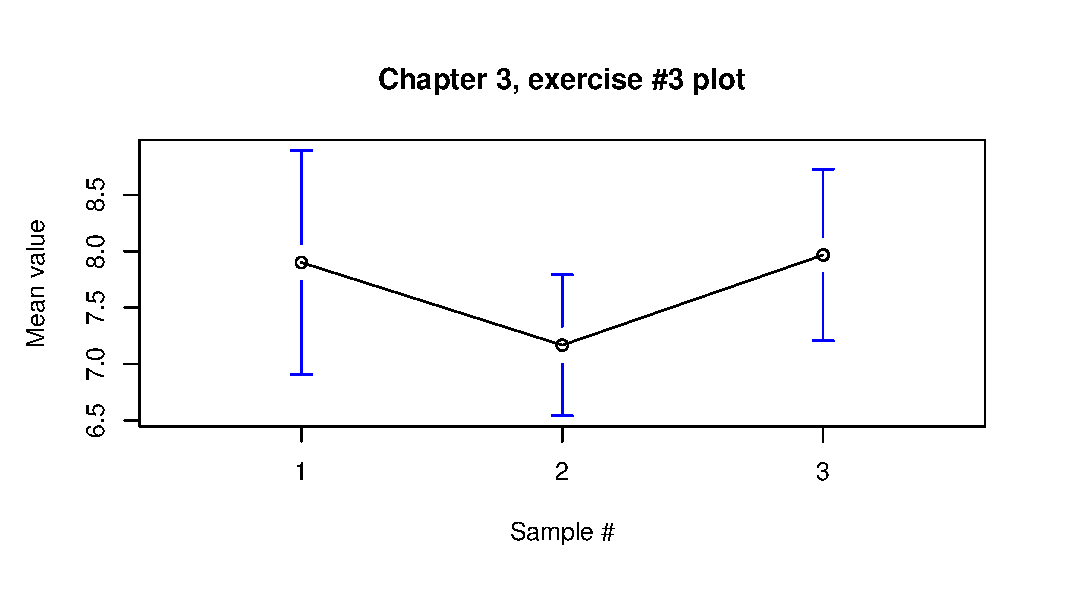
\includegraphics[height=3in, width=\linewidth]{Ex3plot.eps}
	\caption{Plot of mean values with 95\% confidence interval error bars.}\label{Ex3}
\end{figure}
	
\end{enumerate} 
	


\backmatter
% Include the backmatter in the Table of Contents
\cleardoublepage
\addcontentsline{toc}{chapter}{\bibname}

% Bibliography
\printbibliography
\cleardoublepage

% Index
\phantomsection 
\addcontentsline{toc}{chapter}{Index}{}
%\printindex
\begin{theindex}

{\Large\textbf
A
}\hfill\nopagebreak

  \item accuracy\dotfill \hyperpage{8}
  \item average\dotfill \hyperpage{3}, \hyperpage{5}, \hyperpage{8}, 
		\hyperpage{11, 12}, \hyperpage{21}
    \subitem mean\dotfill \hyperpage{5}
    \subitem median\dotfill \hyperpage{5}
    \subitem mode\dotfill \hyperpage{5}

  \indexspace

{\Large\textbf
C
}\hfill\nopagebreak

  \item chemical structure
    \subitem Acid Red 51\dotfill \hyperpage{121}
  \item confidence\dotfill \hyperpage{12, 13}, \hyperpage{17, 18}, 
		\hyperpage{24}, \hyperpage{28}, \hyperpage{114}

  \indexspace

{\Large\textbf
F
}\hfill\nopagebreak

  \item factorial
    \subitem 2x2\dotfill \hyperpage{101}
    \subitem 3x2\dotfill \hyperpage{103}
    \subitem 4x2\dotfill \hyperpage{105}

  \indexspace

{\Large\textbf
H
}\hfill\nopagebreak

  \item hypothesis\dotfill \hyperpage{17, 18}, \hyperpage{21, 22}

  \indexspace

{\Large\textbf
L
}\hfill\nopagebreak

  \item location\dotfill \hyperpage{4--7}, \hyperpage{12}, 
		\hyperpage{18}

  \indexspace

{\Large\textbf
M
}\hfill\nopagebreak

  \item mean\dotfill \hyperpage{5}, \hyperpage{8}, \hyperpage{11}, 
		\hyperpage{17}, \hyperpage{19}, \hyperpage{21}, 
		\hyperpage{23}, \hyperpage{28}, \hyperpage{115}

  \indexspace

{\Large\textbf
N
}\hfill\nopagebreak

  \item null hypothesis\dotfill \hyperpage{18, 19}, \hyperpage{21--24}

  \indexspace

{\Large\textbf
P
}\hfill\nopagebreak

  \item population\dotfill \hyperpage{3}
  \item precision\dotfill \hyperpage{8}

  \indexspace

{\Large\textbf
R
}\hfill\nopagebreak

  \item range\dotfill \hyperpage{7}

  \indexspace

{\Large\textbf
S
}\hfill\nopagebreak

  \item standard deviation\dotfill \hyperpage{3}, \hyperpage{5, 6}, 
		\hyperpage{17}, \hyperpage{23}
  \item statistics
    \subitem inferential\dotfill \hyperpage{4}
    \subitem location\dotfill \hyperpage{5}
    \subitem population\dotfill \hyperpage{3}
    \subitem sample\dotfill \hyperpage{4}
    \subitem variation\dotfill \hyperpage{5, 6}
  \item Student's t Distribution
    \subitem table\dotfill \hyperpage{98}

  \indexspace

{\Large\textbf
T
}\hfill\nopagebreak

  \item t Distribution\dotfill \hyperpage{12}

  \indexspace

{\Large\textbf
V
}\hfill\nopagebreak

  \item variance\dotfill \hyperpage{6}, \hyperpage{8}, \hyperpage{19}
  \item variation\dotfill \hyperpage{7--9}, \hyperpage{12}, 
		\hyperpage{18}

\end{theindex}


\makeatletter
\@openrightfalse
\makeatother

% Colophon
%\include{colophon}

\end{document}
